\chapter{Methods}
\label{Methods}
\section{Project Overview}
To help complete this Master thesis, I created various tools that would help create the final model outputs.
The project is divided into three logical parts, with an optional fourth part.


\subsection{Part 1: Network Creation Tool (GUI)}
\label{sec:part1}
The first part involves the development of a GUI tool to create and edit the network topography of interactions.
This tool allows users to quickly and intuitively define agents, interaction parameters, environmental parameters, and setting parameters.
The tool provides functionalities for adding, editing, and visualizing nodes and edges, as well as importing and exporting the network structure. \newline 
Once the user is happy with the graph shape, they can export the graph for use in part 2 (\Cref{sec:part2}), part 3 (\Cref{sec:part3}), and part 4 (\Cref{sec:part4}). 
The most important part is that the user defines the network edges and the attributes that each node and edge has, as that can't be edited in part 2 onwards. 
It's not a big issue however because the user can upload the graph to the tool again to edit the edge connections and add or remove nodes and attributes. 
In part 3, the user can edit the values of the attributes, so the parameter values do not have to be dialed in, and the user does not need to use the GUI tool to edit parameter values. 


\subsection{Part 2: Simulation Framework}
\label{sec:part2}
The second part focuses on the simulation framework.
The user provides an ODE model and the network topography as input to the framework.
The simulation framework deals with handling the input and output of the data, collecting and storing the data needed for the simulation.
The framework uses SciPy's \textit{solve\_ivp()} numerical solver to simulate the provided ODE equations and calculate the population levels through time.
As output, the user receives two outputs.
The first output is an array of time values that the solver used to calculate the population count.
The second output is an array containing the population count at each time step for every agent.


\subsection{Part 3: Analysis and Visualization}
\label{sec:part3}
The third part involves analyzing and visualizing the simulation results.
The user can use a dashboard built using Plotly Dash to interact with the solver and network.
The user can change parameter, environment values, and setting values on the fly.
This allows the user to quickly change parameter values and test different situations.
The dashboard includes various starter plots that allow the user to test the model.


\subsection{Part 4: Custom Analyses and Visualizations}
\label{sec:part4}
The final part, an optional step, allows for the user to define a number of parameters they want to simulate and download the simulation data after running the simulations. 
Downloading the data then allows the user to create their own custom visualizations without having to rerun the simulations, especially if there are many long and complex simulations. 
The data can then be further processed and visualized as the user wishes. 


\section{Network Topography of Interactions Creation Tool}
Numerous interactions are occurring between agents in a microbial environment.
However, not every agent can and will interact with one another.
Based on which agents interact with one another, a network topography can be created, capturing the dynamics of the interactions.
Every node represents a unique agent, and each agent has their own intrinsic properties. 
This would include the starting population or concentration, reproduction rate, and death rate. \newline 

An edge links agents together if there is an arbitrary interaction occurring between two agents, with the properties exhibited in the interaction dependent on the interacting agents. 
Self interactions are allowed in the network. 
Large populations of bacteria can provide support to other bacteria and prevent phage infection. 
Each edge likewise also contains attributes to capture the unique dynamic interactions between the agents.
This could be the probability for a successful interaction, the burst size of a specific phage-bacteria pair, or the bacteria's consumption rate of resources.
Adding the attributes to the nodes and edges allow for the capture of various interaction dynamics within the context of the community.


A GUI tool has been developed using Python and NetworkX to help aid in the development of the exhibited network topography.
With this tool, a network topography can be created by adding any number of phages, bacteria, and resources. 
There is an environment node that is used to store global environmental data, for example, the temperature of the system, the pH of the system, the wash-in/out rate, etc.
The settings node holds information such as simulation length, max time step, and the type of ODE solver to use.
The interactions and attributes of the agents, environment, and settings can easily be edited using the GUI tool. 

\Cref{fig:ss:initial_startup_GUI_tool} shows the layout of the GUI tool built using Tkinter and NetworkX. \Cref{fig:ss:example_network} shows an example network that can be created. %TODO: Citation needed.
There are numerous buttons that can be used to edit the graph, for example adding or removing nodes and edges. 
By default, an environment node holding parameters such as pH and temperature is added.
A settings node is added as well, holding settings data to be used for the solver, like the type of solver or simulation length.
Manually adding nodes and edges can get tedious and repetitive for large graphs, so the user can add multiple nodes and edges at the same time.
Nothing can interact with the environment and setting node, as they are used to hold data about the environment and network solver.
For each node and edge, default attribute names and values are added which can later be edited by the user. 
The user can alter the default attribute name and value by importing the GUI tool class and overriding the method implementation implementing the default names and values. 
The nature of the interaction needs to be defined and captured in the parameter names, values, and ODE equations.

\begin{figure}
    \centering
    \begin{subfigure}{0.49\linewidth}
        \centering
        \vspace*{\fill}
        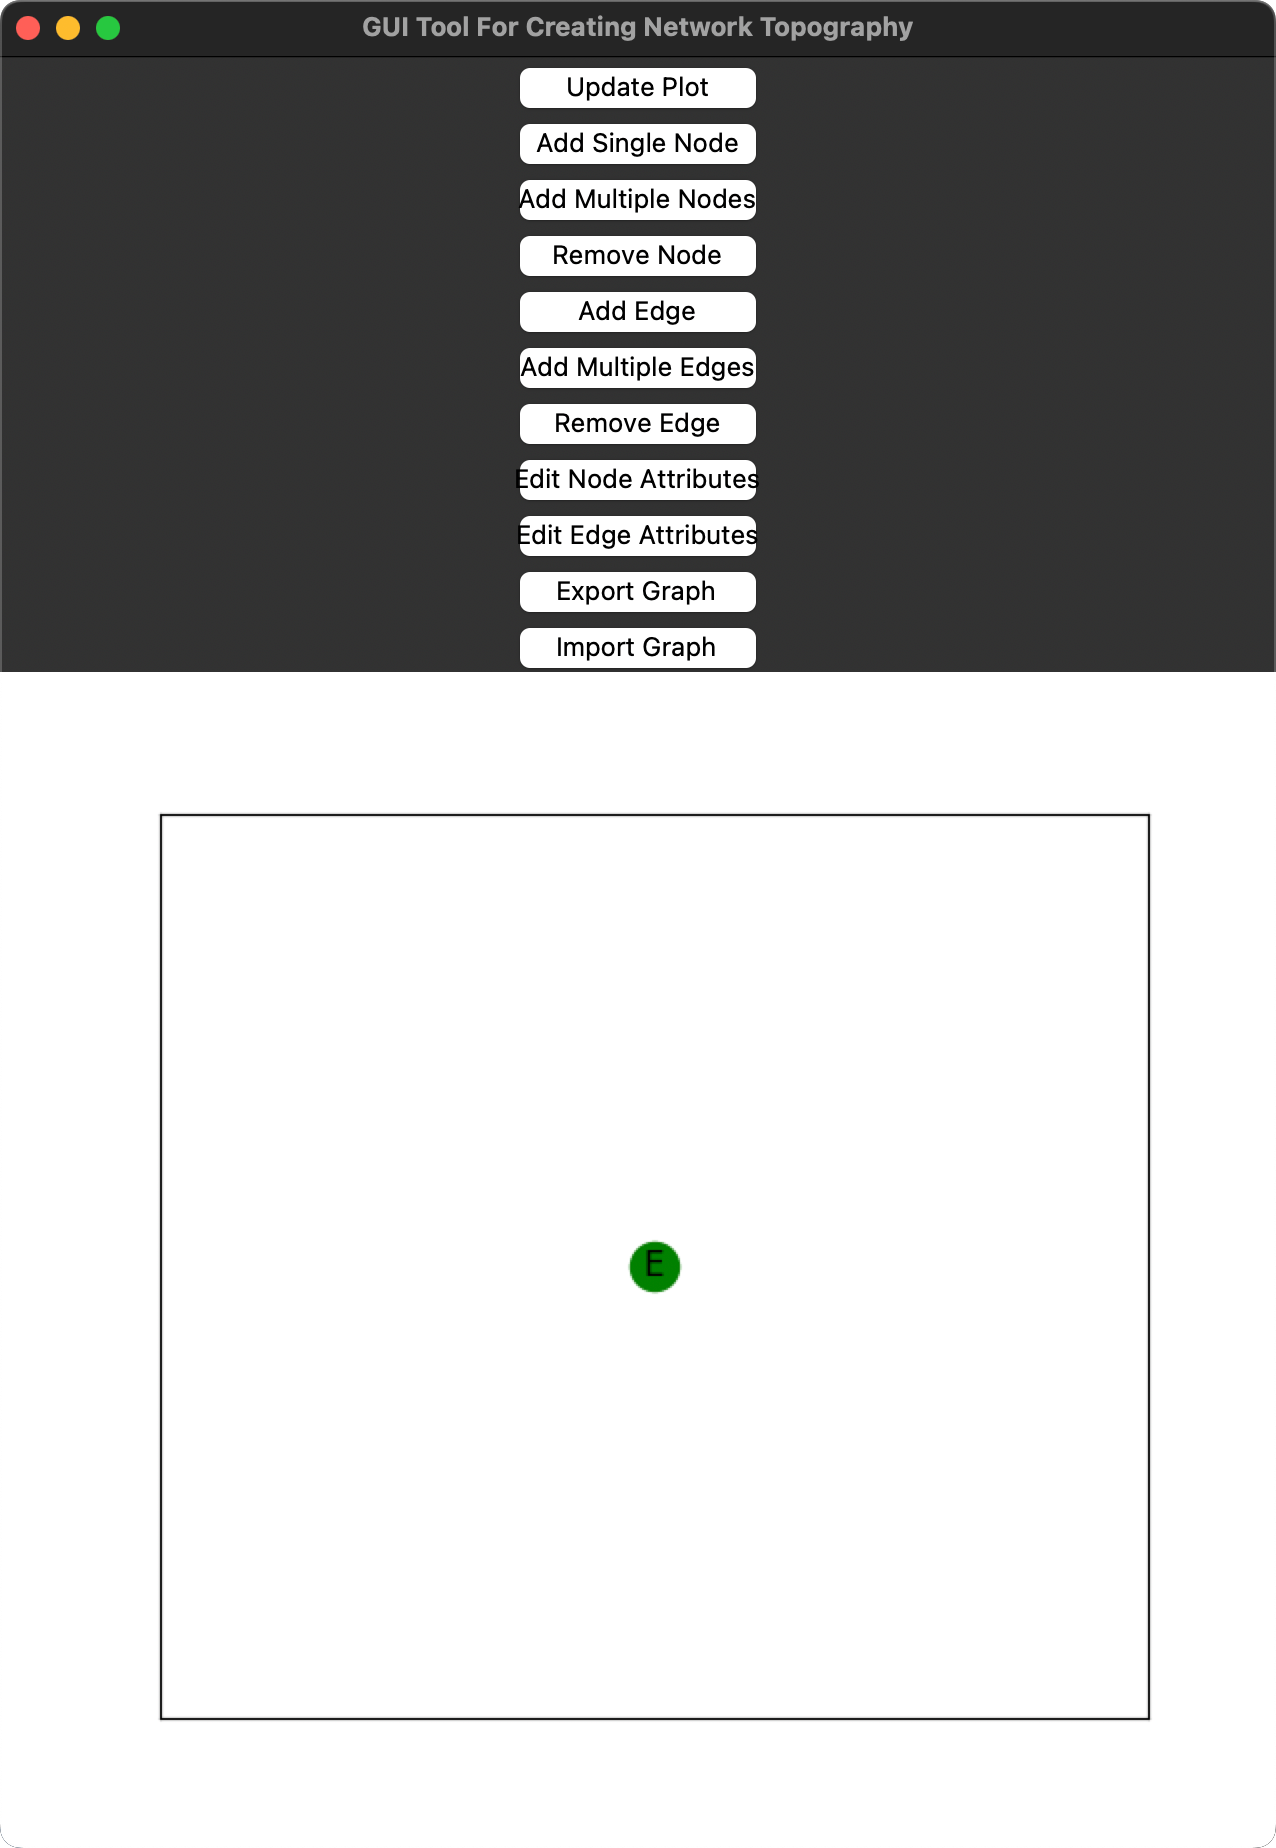
\includegraphics[width=\linewidth]{Screenshots/initial_startup_GUI_tool.png}
        \caption{
            The GUI tool as seen on the startup of the program.
        }
        \label{fig:ss:initial_startup_GUI_tool}
        \vspace*{\fill}
    \end{subfigure}
    \begin{subfigure}{0.49\linewidth}
        \centering
        \vspace*{\fill}
        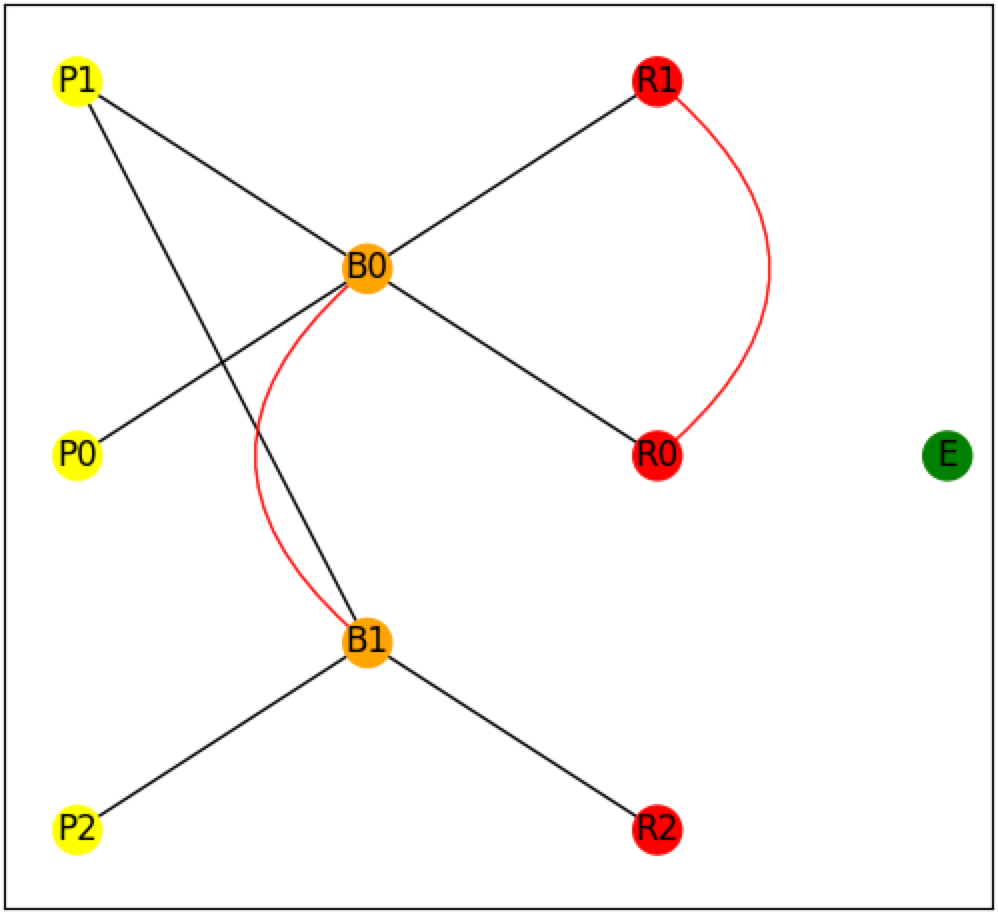
\includegraphics[width=\linewidth]{Screenshots/example_network.png}
        \caption{
            An arbitrary $3\times2\times3$ network with each node representing a phage, bacteria, or resource, with arbitrary interactions occurring between them. 
        }
        \vspace*{\fill}
        \label{fig:ss:example_network}
    \end{subfigure} 
 \end{figure}

\section{Dashboard for Analysis and Visualization}
The dashboard allows the user to interact with the network, the model, and some prebuilt visualizations, and is built into three logical sections.
The first section allows for the user to edit the network parameters and setting values on the fly to quickly iterate through different conditions and to fine-tune parameter selection without having to rebuild the network using the GUI tool.
The second section allows for the user to see how the population count evolves over time for a given initial condition and parameter values, allowing to quickly test the network input.
The final section allows for the user to run more advanced analyses on the network, for example, by changing multiple parameter values and visualizing the output. 

\subsection{Editing Network and Parameter Values}
\label{sec:editing_network_and_parameter_values}
The editing network and parameter value contain five separate sections.
\paragraph{Initial Condition}
The initial condition settings panel (\Cref{fig:ss:ds:initial_condition}) allows for the user to edit the initial starting values of the agents. 
Each agent type has a table containing the initial population count. 
Extra hidden agents can be included. 
When a bacteria has been infected, the bacteria goes through multiple stages before lysing. Each bacteria agent starts out as uninfected, and once infected, the bacteria goes through 4 stages of infection before lysing as seen in \Cref{fig:ss:ds:initial_condition}. \newline 
\paragraph{Vector Data} 
Data that can be represented as a vector, for example the data attributed to an agent type have their own section, \Cref{fig:ss:ds:vector}.
\paragraph{Matrix Data}
Data that is stored as a matrix, the data stored on edges between agents, is stored in the matrix tab (\Cref{fig:ss:ds:matrix}).
\paragraph{Environment and settings}
The environment data and settings data also have their own tab, \Cref{fig:ss:ds:environment} and \Cref{fig:ss:ds:settings} respectively.

\begin{figure}[h!]
    \centering
    \begin{subfigure}{0.49\linewidth}
        \centering
        \vspace*{\fill}
        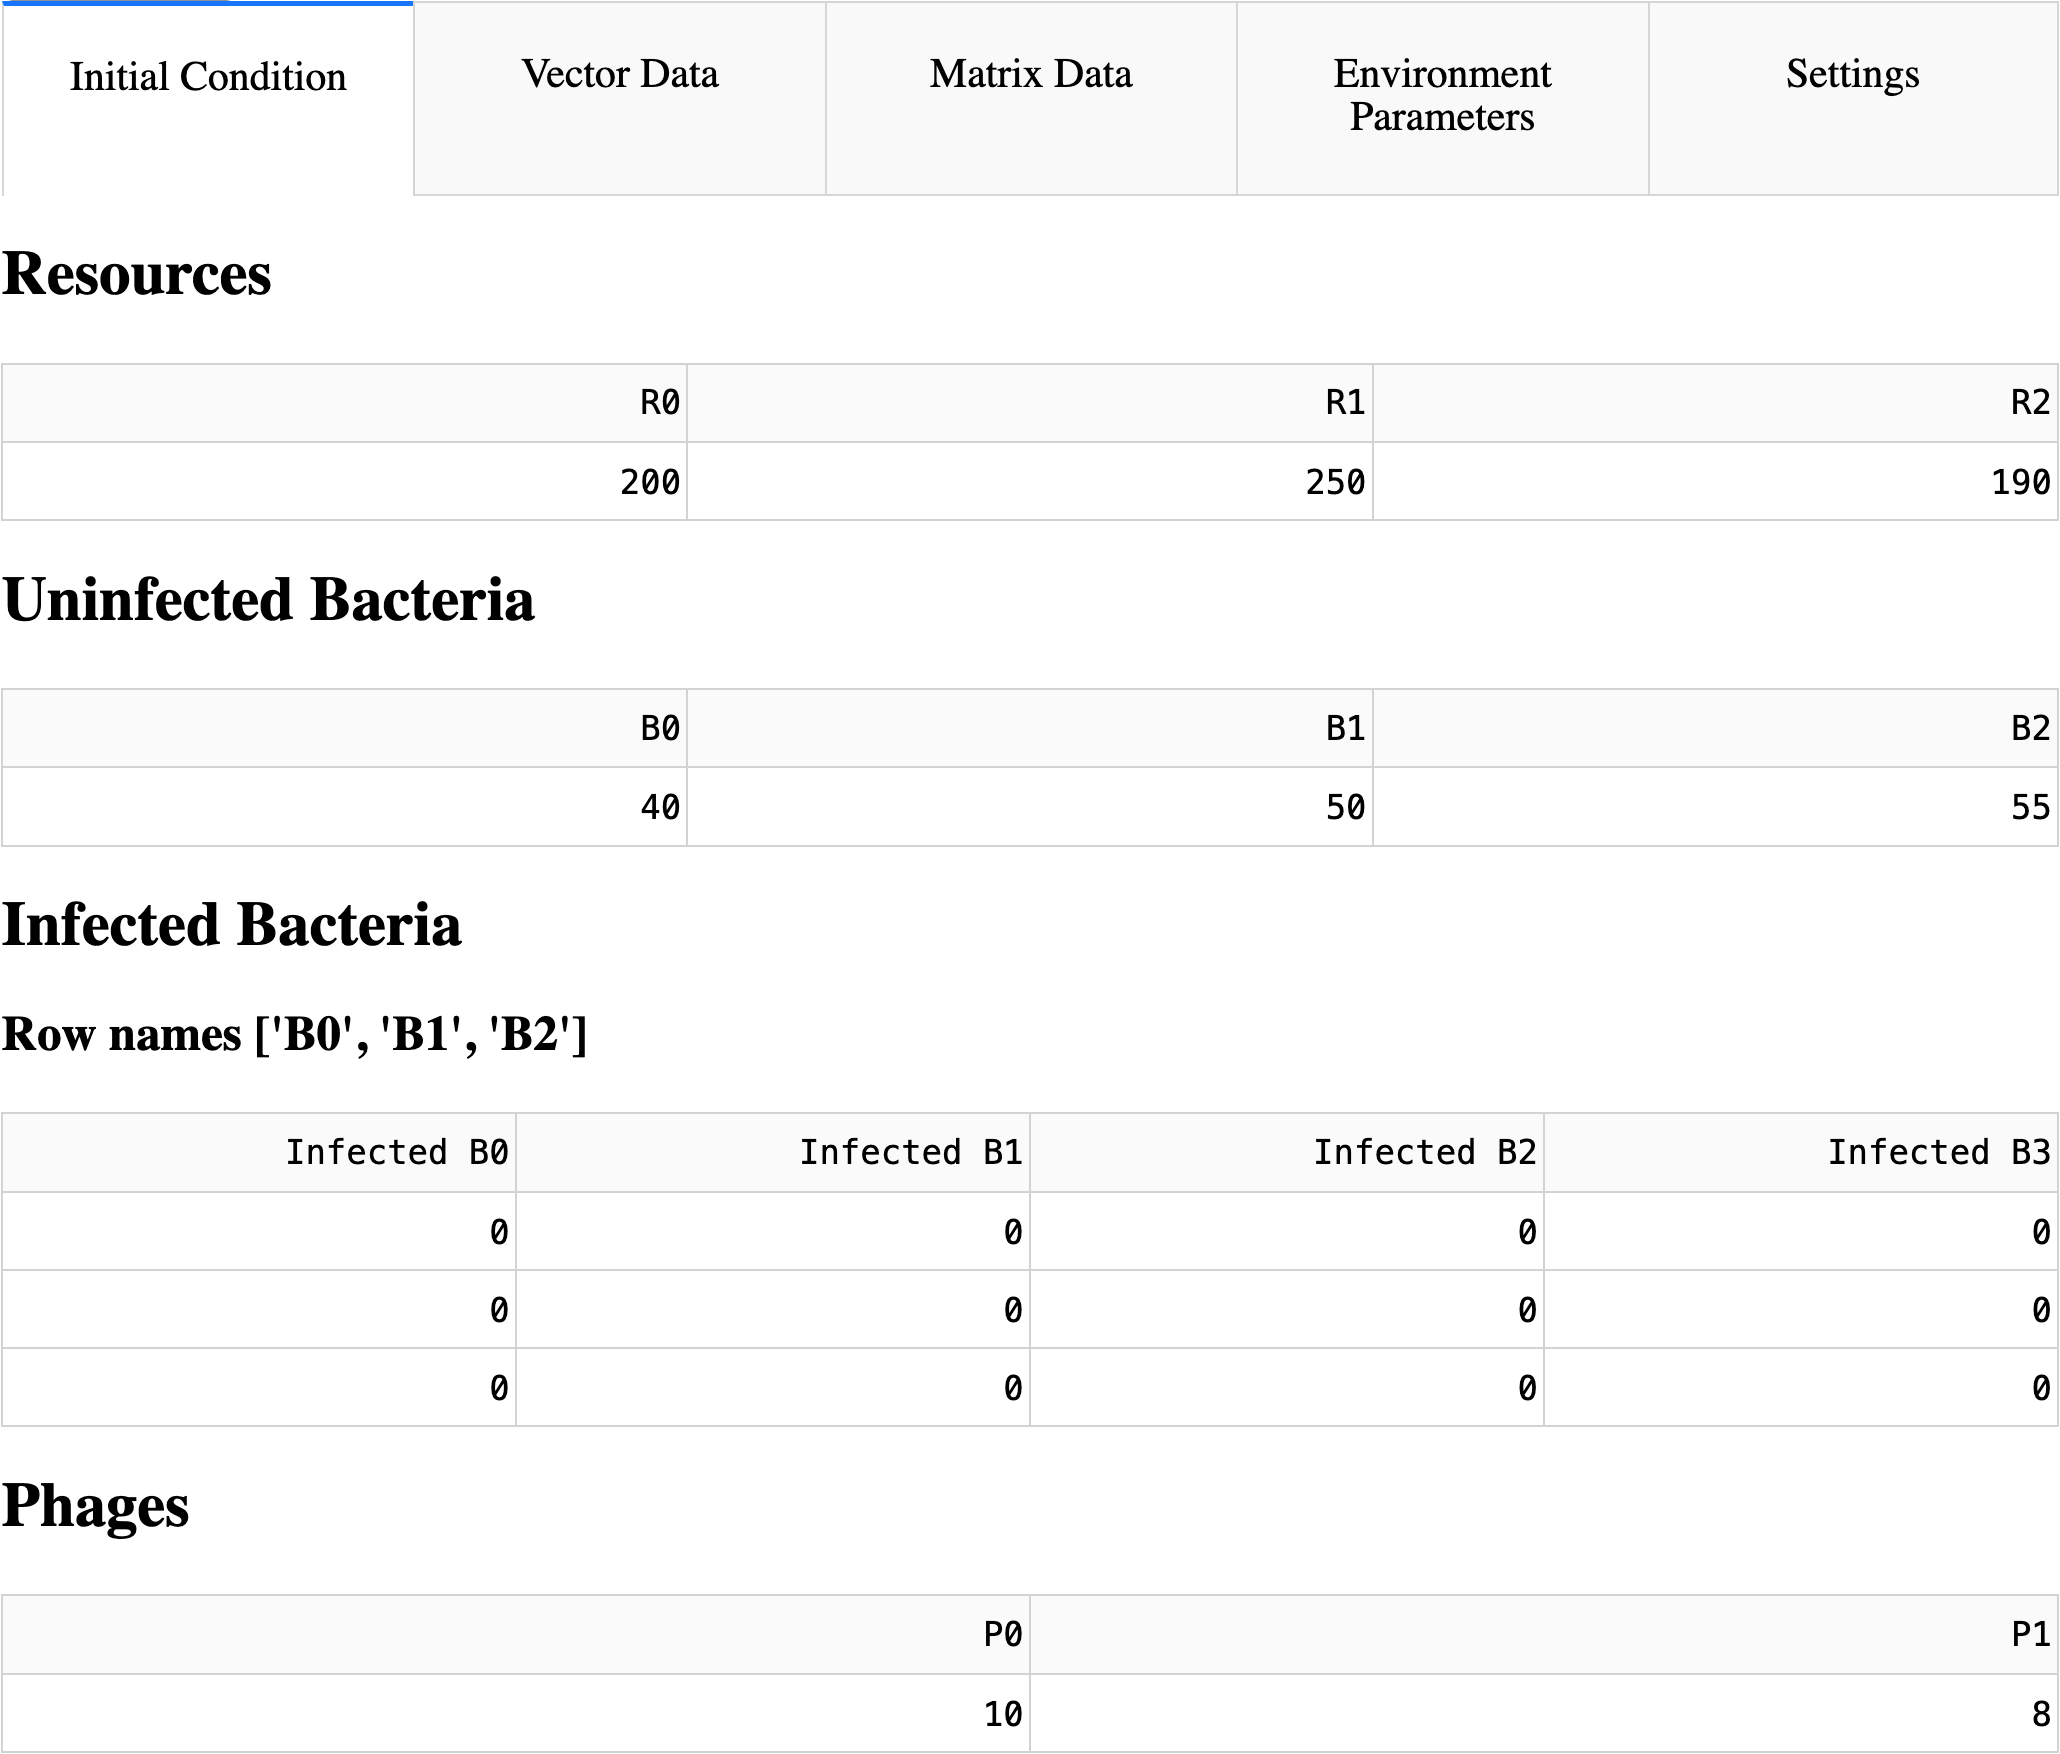
\includegraphics[width=\linewidth]{Screenshots/DashboardSettings/initial_condition_settings.png}
        \caption{
            The tab where the user can edit the initial conditions of the agents.
        }
        \label{fig:ss:ds:initial_condition}
        \vspace*{\fill}
    \end{subfigure}
    \hfill
    \begin{subfigure}{0.49\linewidth}
        \centering
        \vspace*{\fill}
        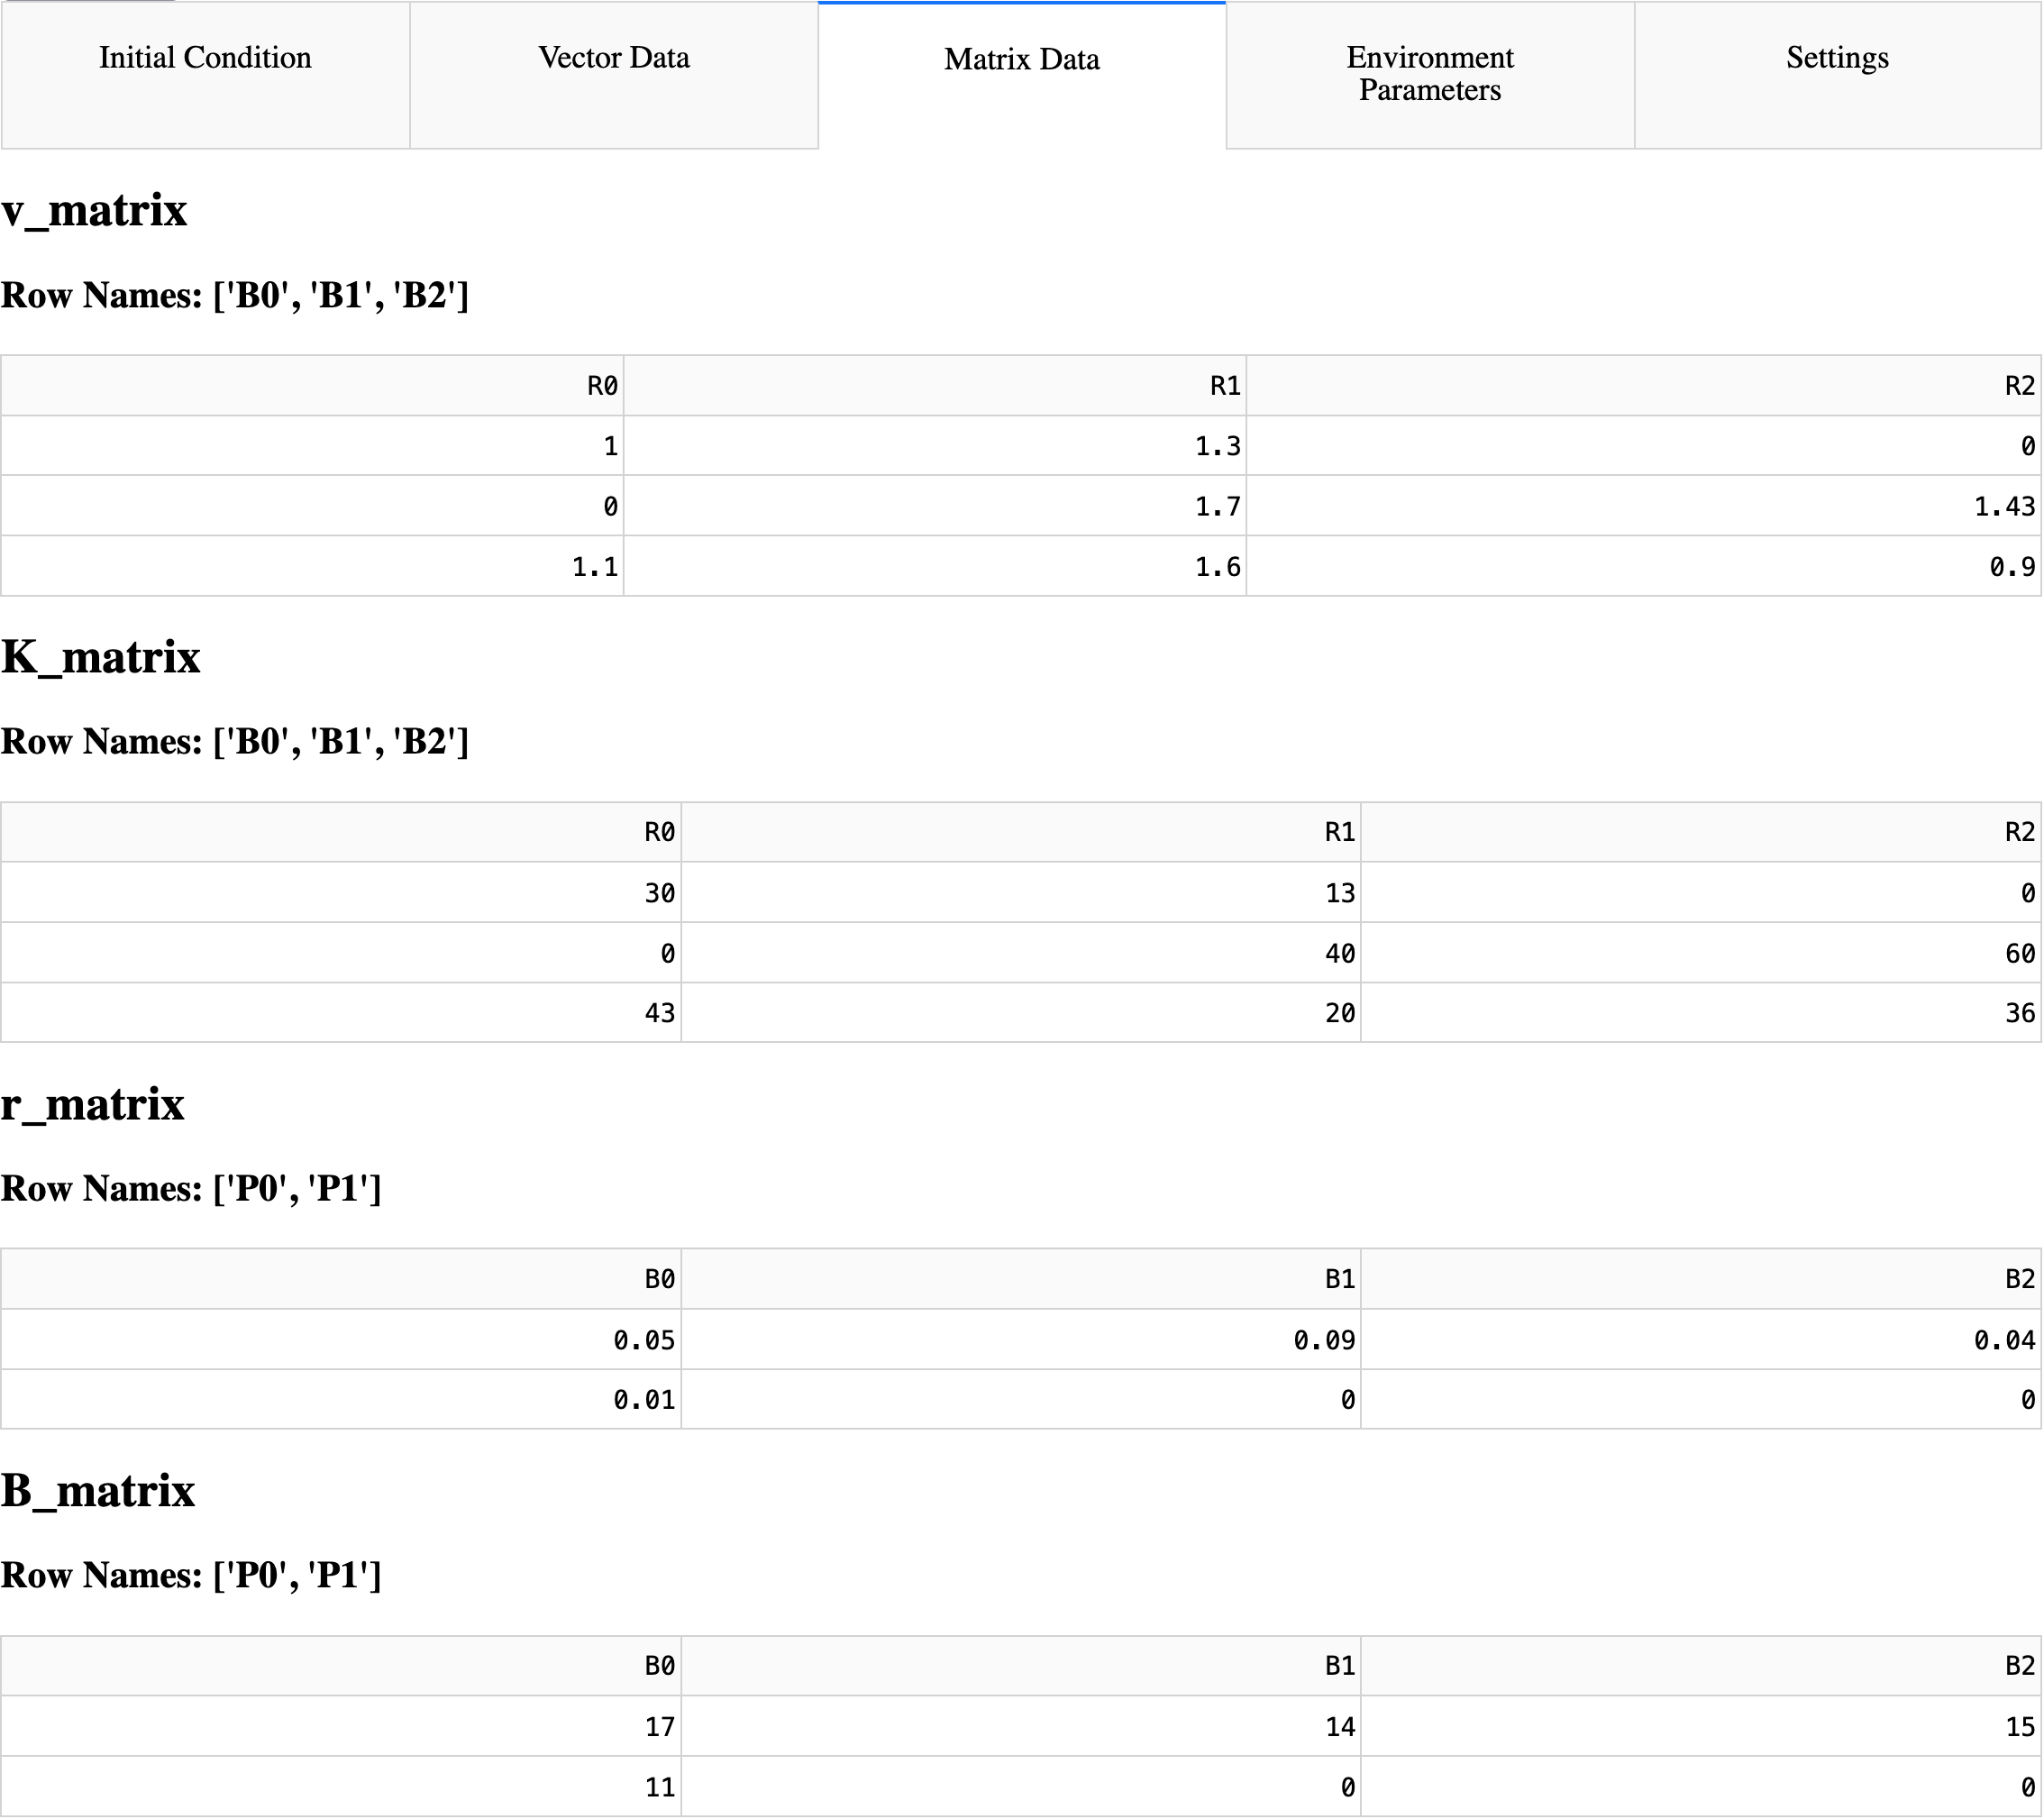
\includegraphics[width=\linewidth]{Screenshots/DashboardSettings/initial_matrix_settings.png}
        \caption{
            The tab where the user can edit the matrix attribute values. 
        }
        \label{fig:ss:ds:matrix}
        \vspace*{\fill}
    \end{subfigure}
    \hfill
    \begin{subfigure}{0.49\linewidth}
        \centering
        \vspace*{\fill}
        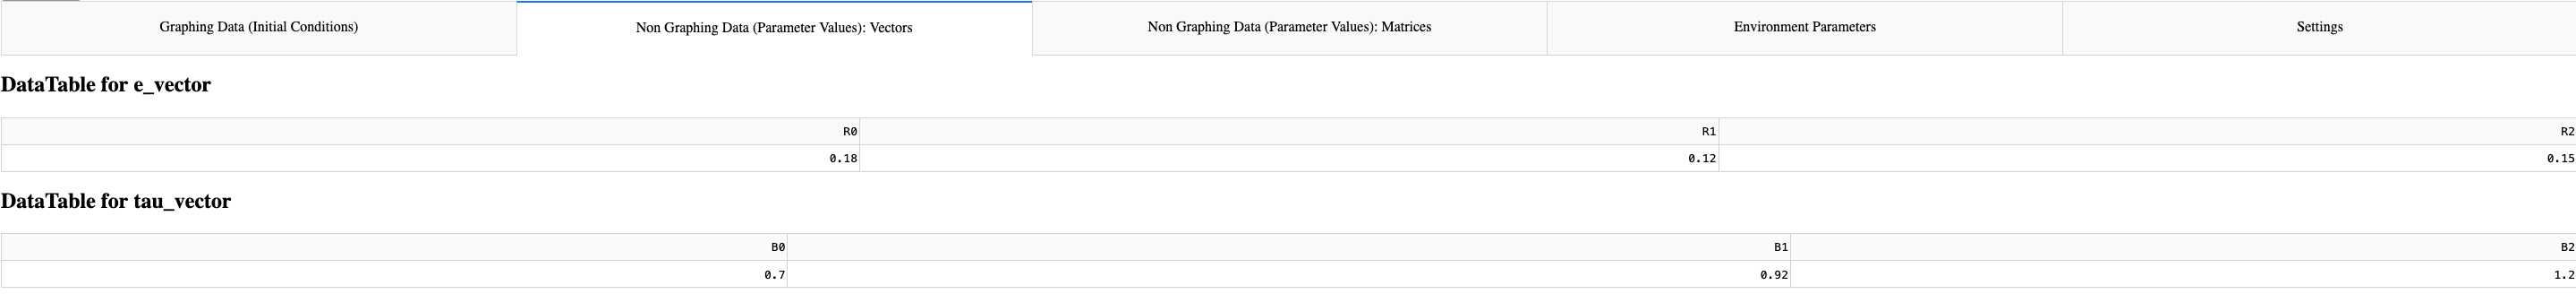
\includegraphics[width=\linewidth]{Screenshots/DashboardSettings/initial_vector_settings.png}
        \caption{
            The tab where the user can edit the vector attribute values.
        }
        \vspace*{\fill}
        \label{fig:ss:ds:vector}
    \end{subfigure}
    \hfill
    \begin{subfigure}{0.49\linewidth}
        \centering
        \vspace*{\fill}
        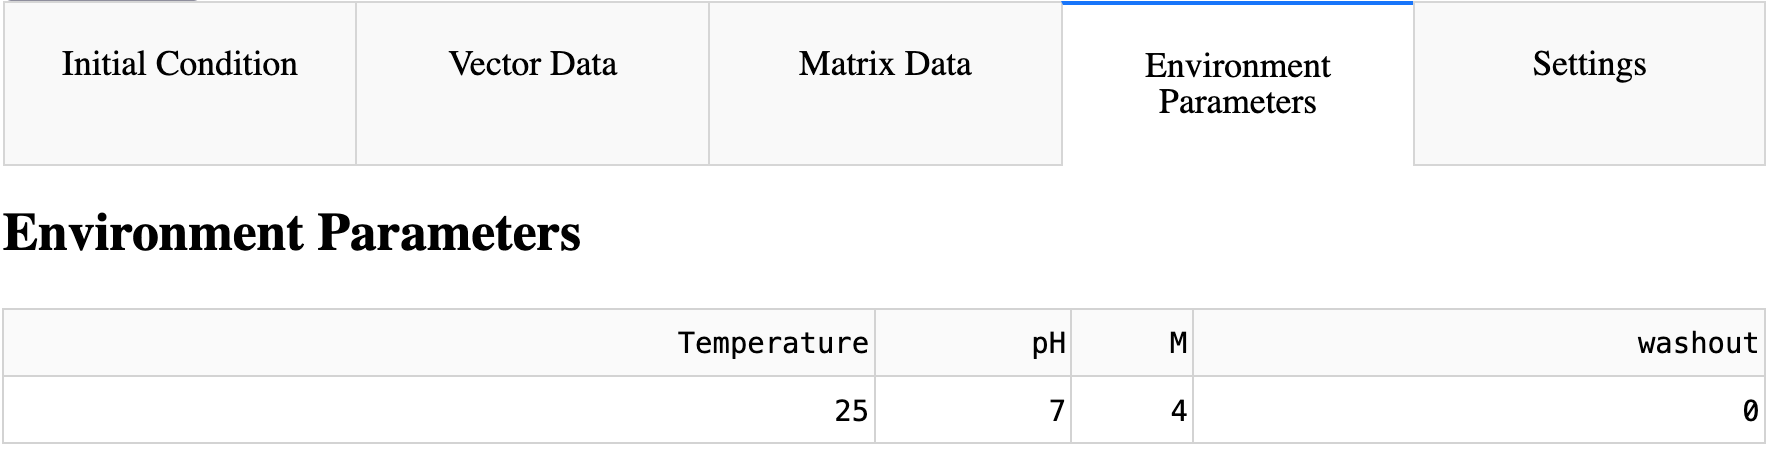
\includegraphics[width=\linewidth]{Screenshots/DashboardSettings/initial_environment_settings.png}
        \caption{
            The tab where the user can edit the environment values. 
        }
        \label{fig:ss:ds:environment}
        \vspace*{\fill}
    \end{subfigure}
    \hfill
    \begin{subfigure}{0.49\linewidth}
        \centering
        \vspace*{\fill}
        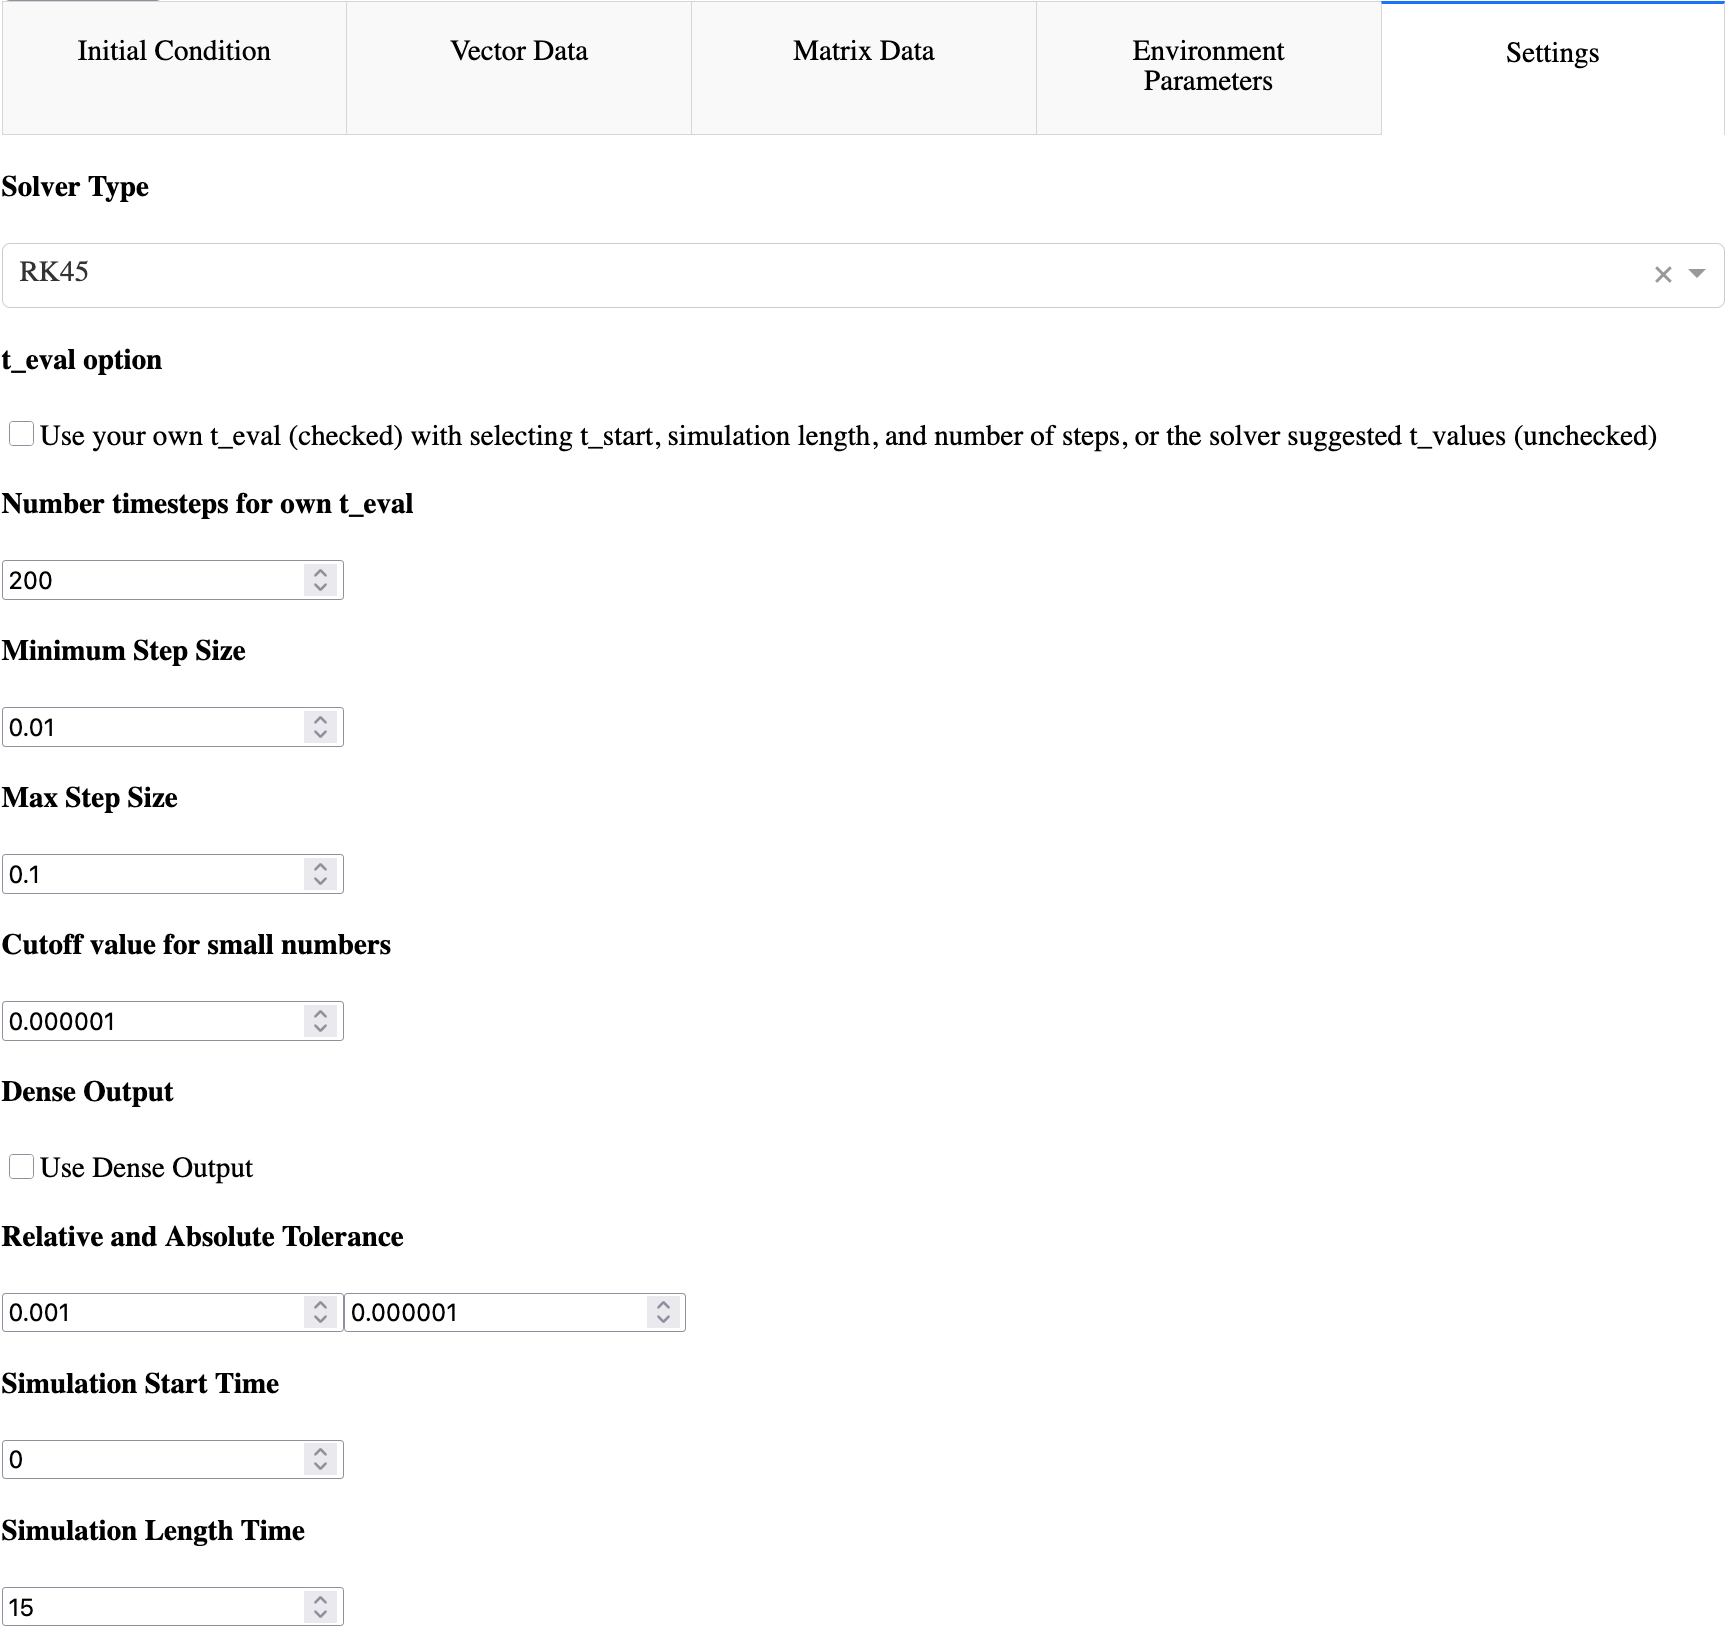
\includegraphics[width=\linewidth]{Screenshots/DashboardSettings/initial_settings_settings.png}
        \caption{
            The tab where a user can edit the settings of the solver and simulation. 
        }
        \label{fig:ss:ds:settings}
        \vspace*{\fill}
    \end{subfigure}
    \caption{The tabs where the user can edit the various parameter values and control the simulation parameters}
 \end{figure}

\subsection{Advanced Visualization and Analysis}
In the advanced analysis section, the user can run different analysis methods to gain a greater understanding of the model.
The visualizations only support a $1 \times 1\times 1$ model, in order to make the analysis easier for the user, and to make it easier to analyze the visualization.
These advanced visualizations were created with the mind of understanding a simple network.
There are five different analysis and visualization methods, and one system where the user can run a large simulation on the whole network and receive an output file containing the raw simulation file data.
The raw data is stored as a \textit{parquet} file, a tabular-like data format, which when combined with Dask (not Dash), allows for querying of the data similarly to Pandas.
Parquet with Dask offers superior performance and data storage solutions that Pandas can't offer.
Once queried, the user can create their own graphs and plots as they have access to the parameter values used and the raw simulation data.

\subsubsection{Serial Transfer}
\label{sec:serial_transfer}
Serial transfer is a method employed by bacteriologist where after a set amount of time, the bacteriologist pipettes a specified amount of media (for example 10ml of liquid) containing bacteria and resources, possibly with phages, and transfers the old media into a solution containing new media.
At this stage, the bacteriologist can introduce new agents, or re-introduce agents if the agent population or concentration has died out.
However, usually only resources are added during the transfer process.
An example would be an experiment starts with 50ml of solution.
The experiment runs for 24 hours before 5ml is removed.
Researchers can run various tests, such as using optical density measurements to assess bacterial density in the solution or employing a mass spectrometer to determine the concentration of the resources.
The 5ml is then re-added to a new solution of 45ml containing fresh resources.
The effect that this has is it creates a sort of artificial stable point.
As the bacteria grow, they consume the resources found in the solution.
However eventually the resources run out, and the bacteria die out due to a lack of resources.
By introducing new resources at set time intervals, the bacteria can regrow and exhibit a semi-stationary behavior.
\newline

The implementation of serial transfer is slightly different.
A user can select a number which will divide the population count of the agents by that number (\Cref{fig:ss:av:serial_transfer_settings}).
Then the program takes the initial condition values defined for the resources the initial condition in \Cref{sec:editing_network_and_parameter_values} and adds those values to the resources respectively.
By selecting a checkbox, the values as defined in the initial condition box for phages and bacteria in \Cref{sec:editing_network_and_parameter_values} can optionally be added as well.
As an example, if at the end of a simulation, there are 120 resources, 5000 bacteria, and 1000 phages remaining and the chosen serial transfer value is 15, then the resource, bacteria, and phage values would be decreased to 8, 333.33, and 66.66 respectively.
Then, if the initial condition for the resources, bacteria, and phages in \Cref{sec:editing_network_and_parameter_values} are 500, 80, and 10 respectively, and the checkbox is unchecked, the new population count will be 508, 333.33 and 66.66 respectively.
If the checkbox is checked, the new population count will be 508, 413.33, and 76.66 respectively.
These new values would be used as the new starting initial condition for a new simulation, and the run results will be appended to the previous run.
As output, new graphs are created showing the runs appended to one another, with an example output shown in \Cref{fig:ss:av:serial_transfer_run}.

\begin{figure}[h!]
    \centering
    \begin{subfigure}{0.49\linewidth}
        \centering
        \vspace*{\fill}
        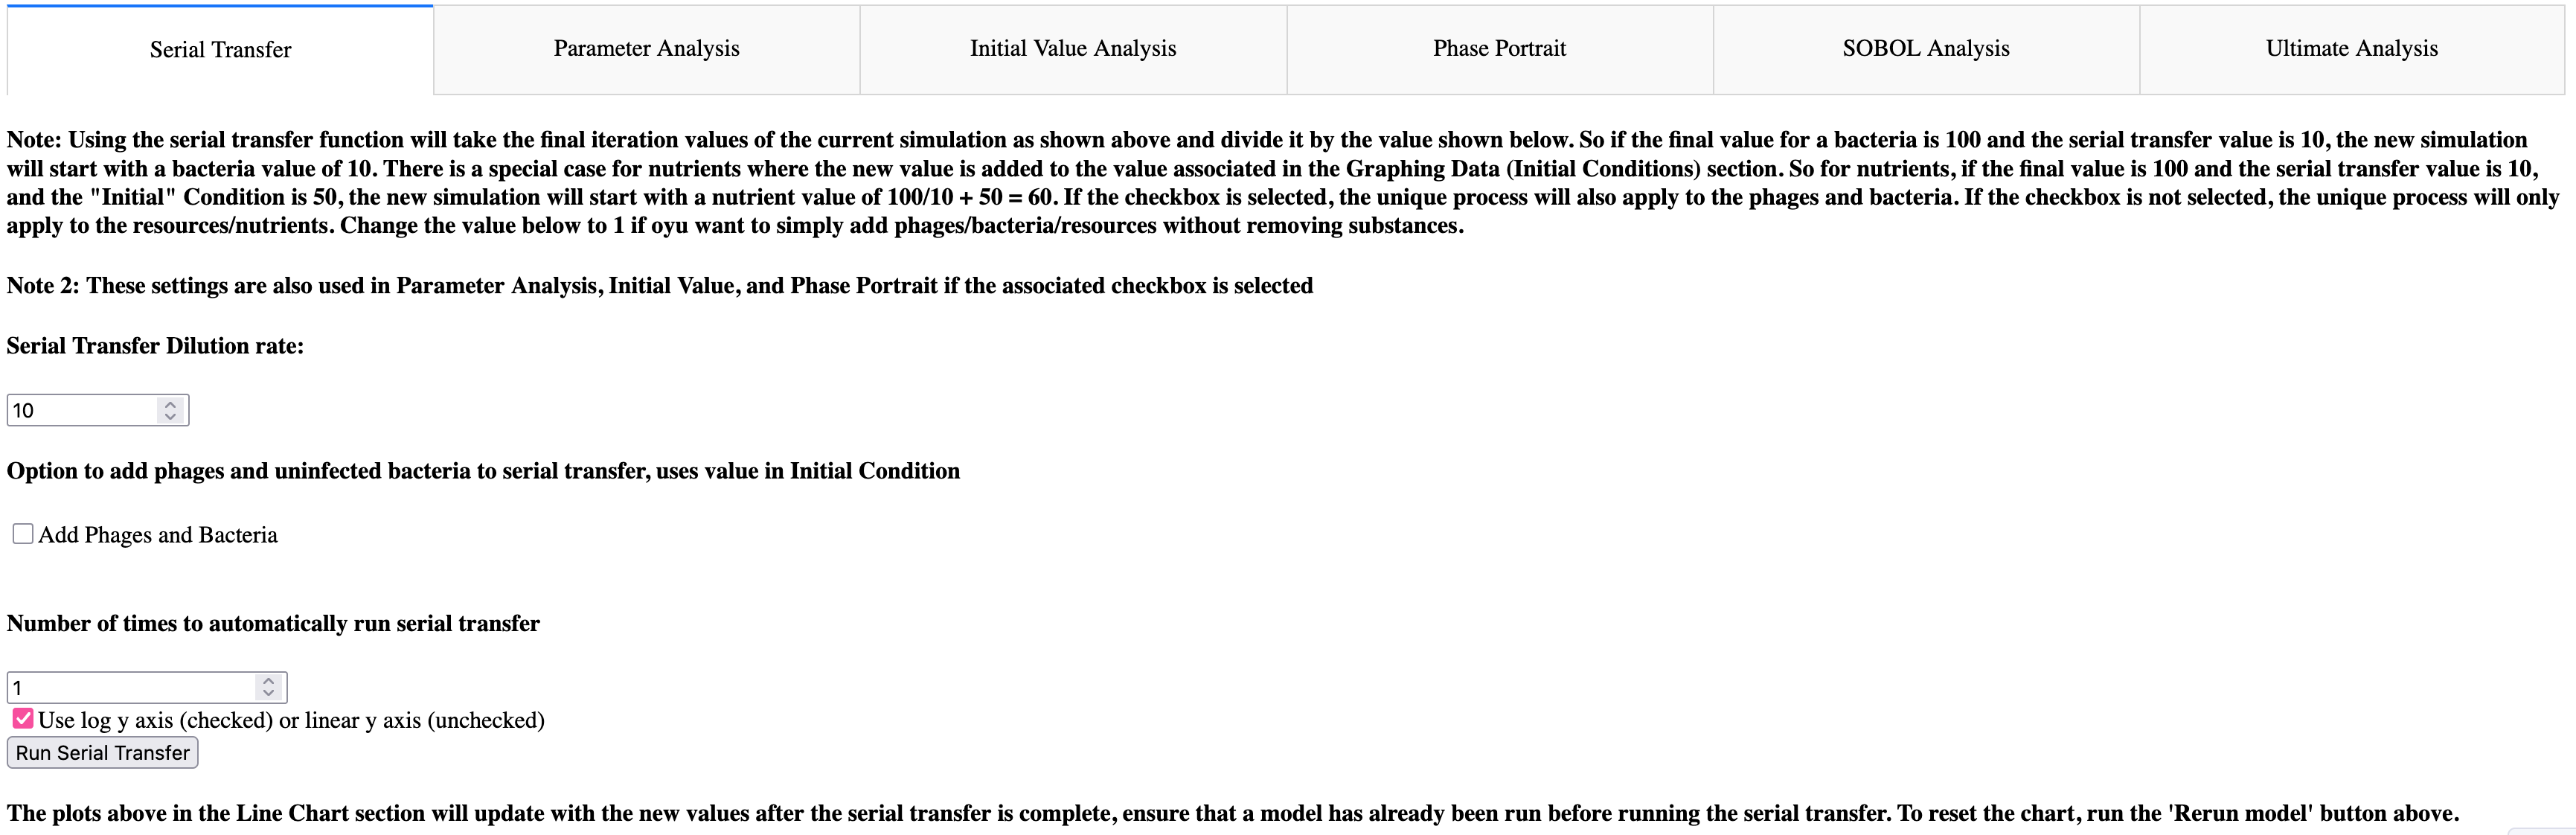
\includegraphics[width=\linewidth]{Screenshots/AdvancedVisualization/serial_transfer_settings.png}
        \caption{
            The section where the user can set up the serial transfer.
        }
        \label{fig:ss:av:serial_transfer_settings}
        \vspace*{\fill}
    \end{subfigure}
    \hfill
    \begin{subfigure}{0.49\linewidth}
        \centering
        \vspace*{\fill}
        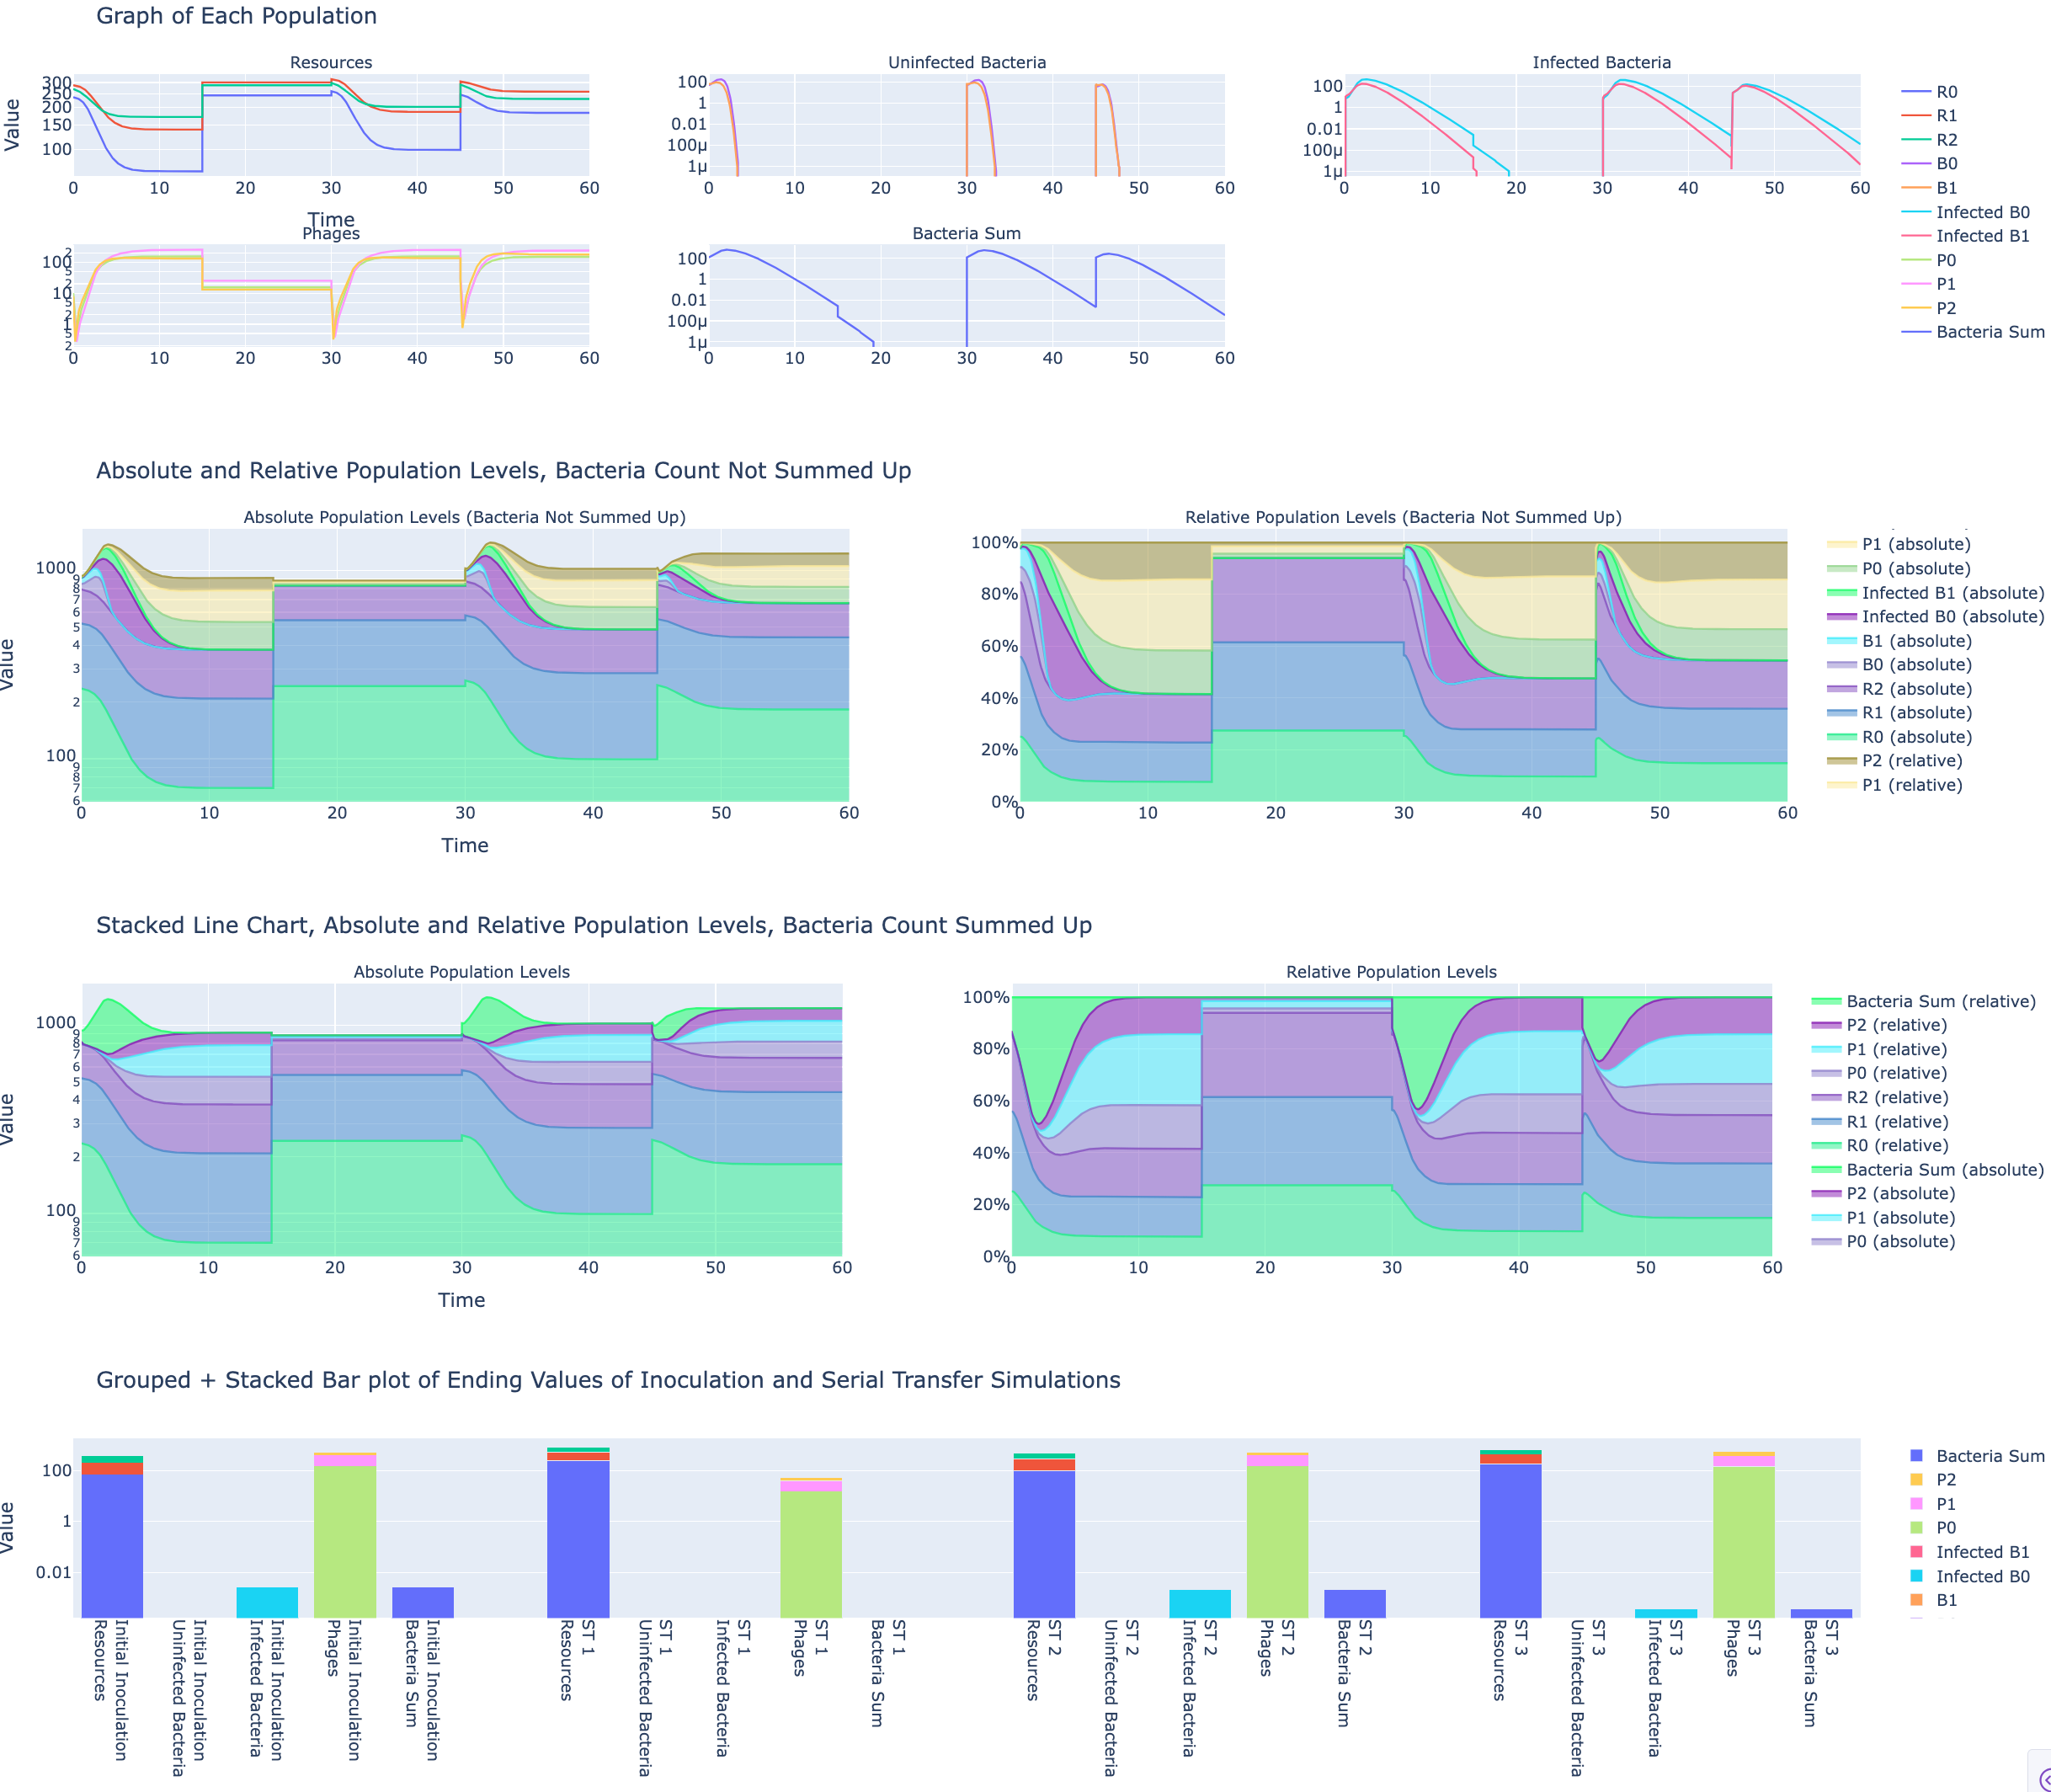
\includegraphics[width=\linewidth]{Screenshots/AdvancedVisualization/serial_transfer_run.png}
        \caption{
            The output plots of serial transfer. 
        }
        \label{fig:ss:av:serial_transfer_run}
        \vspace*{\fill}
    \end{subfigure}
    \caption{Serial Transfer}
 \end{figure}

\subsubsection{Parameter Analysis}
\label{sec:parameter_analysis}
The parameter analysis settings tab as shown in \Cref{fig:ss:av:parameter_analysis_settings} allows the user to choose two parameters and individually run the model with the varying input values.
The values that can be tested and changed include all initial condition values, vector and matrix data, and environmental data.
As input, the user can select 2 parameters of choice.
After the parameter name selection, the user can manually choose which parameter values they want to test or test a range of values equally spaced by selecting the number of values to test.
Finally, the user can optionally run a serial transfer, where the serial transfer uses the settings found on the Serial Transfer tab. \newline

\Cref{fig:ss:av:parameter_analysis_run} shows the heatmap that the user can expect, one heatmap for each agent type.
Each heatmap has cells that unique model input, and contains the value of
A heatmap matrix is created for each agent type, with dimension of the input values.
Each box corresponds to each pair of parameter inputs, and shows the population count of the agent at the time selected on the slider. 
As the user slides the slider, the value inside the cell changes to correspond with the chosen time. 
Note that the heatmap color range resets for each heatmap, so similar colors across heatmaps will not correspond to the same values.

\begin{figure}[h!]
    \centering
    \begin{subfigure}{0.49\linewidth}
        \centering
        \vspace*{\fill}
        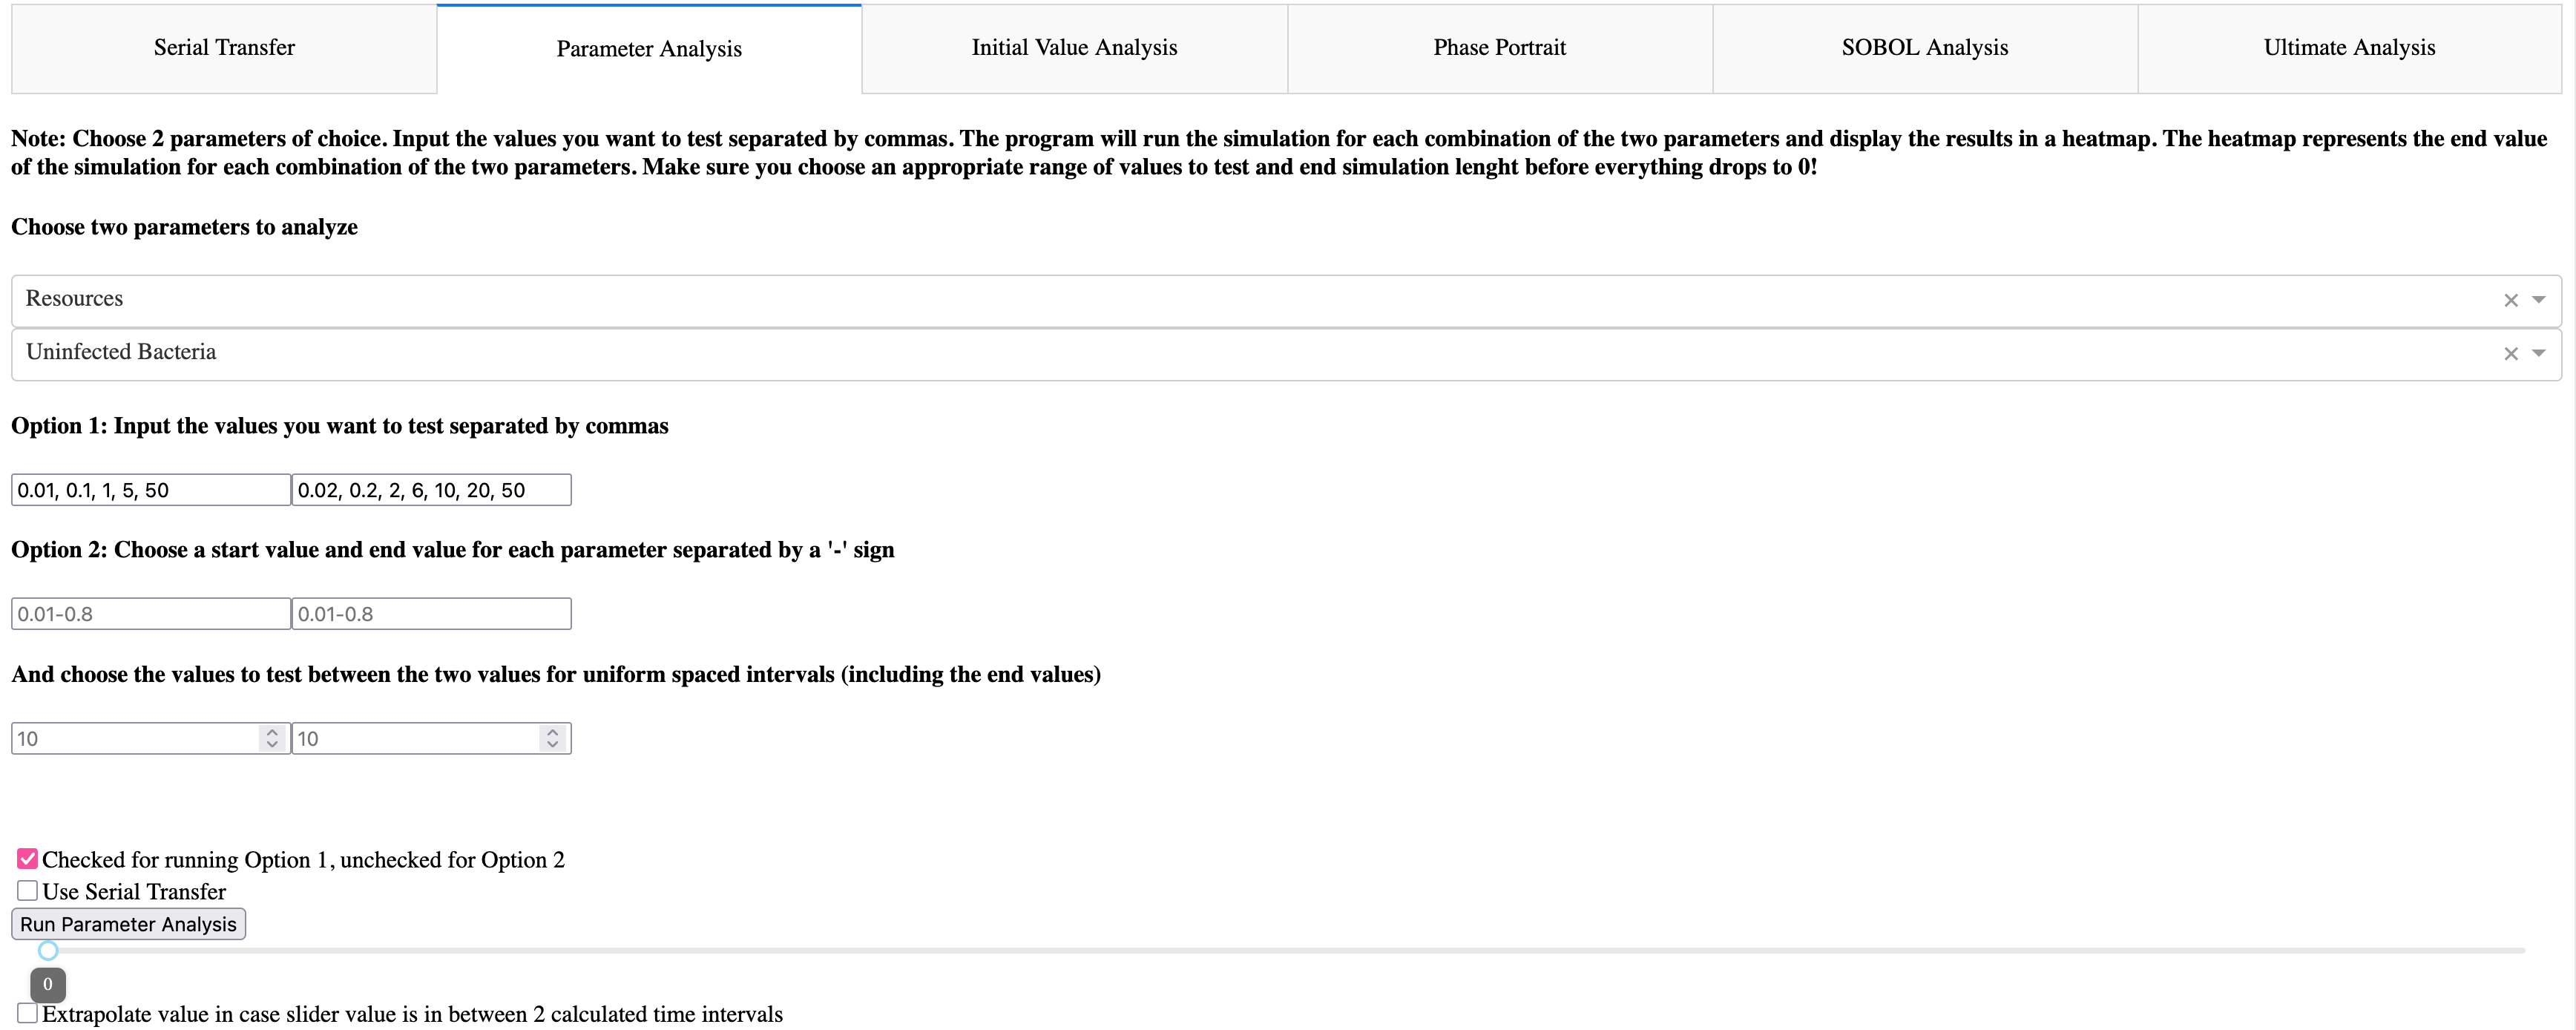
\includegraphics[width=\linewidth]{Screenshots/AdvancedVisualization/parameter_analysis_settings.png}
        \caption{
            The options available for the parameter analysis. 
        }
        \label{fig:ss:av:parameter_analysis_settings}
        \vspace*{\fill}
    \end{subfigure}
    \hfill
    \begin{subfigure}{0.49\linewidth}
        \centering
        \vspace*{\fill}
        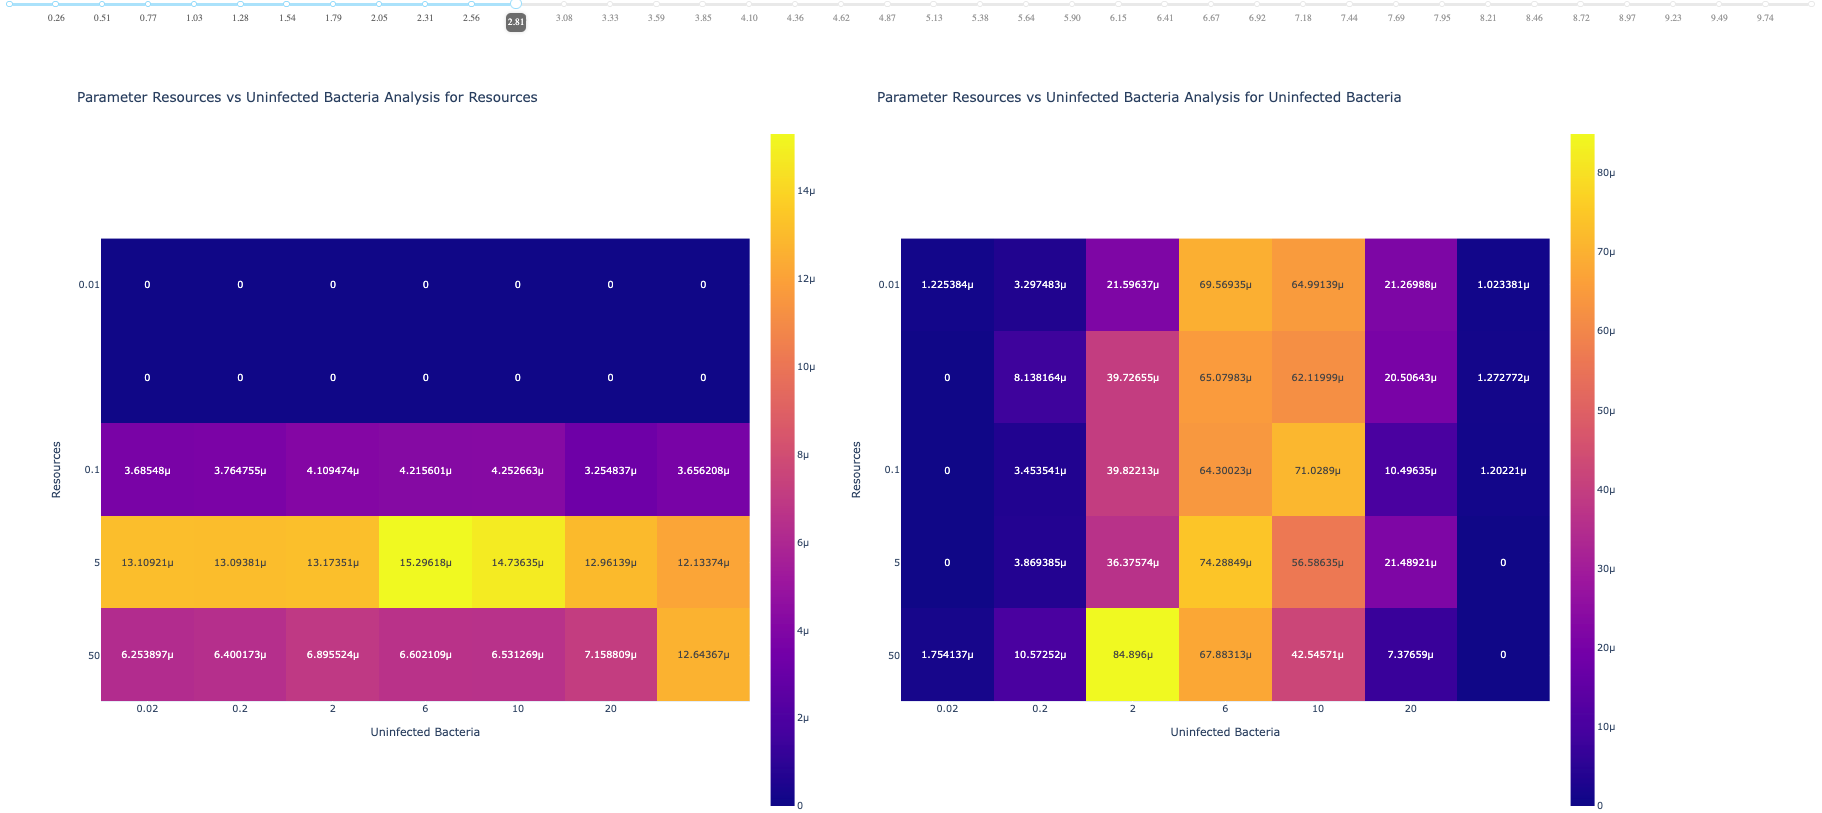
\includegraphics[width=\linewidth]{Screenshots/AdvancedVisualization/parameter_analysis_run.png}
        \caption{
            The output that the user can expect
        }
        \label{fig:ss:av:parameter_analysis_run}
        \vspace*{\fill}
    \end{subfigure}
    \caption{Parameter Analysis}
\end{figure}


\subsubsection{Initial Value Analysis}
\label{sec:initial_value_analysis}
The initial value analysis settings tab as shown in \Cref{fig:ss:av:initial_value_analysis_settings} allows the user to choose a single parameter and vary the value of that parameter, visualizing how a change in parameter value affects the population count of the agents.

\Cref{fig:ss:av:initial_value_analysis_run} shows the plots that the user receives.
For each agent type, there are three plots made.
The left plot shows the population count through time, one line for each parameter value submitted.
The middle plot takes each run and calculates the “percentage from the max value“ (default value of $0.95 \rightarrow 95\%$) reached of the peak.
This value is considered the time of peak, and is used to fix some issues that can arise where the population plateaus or only keeps on rising.
The initial value is plotted on the x-axis, with the time at which the max value is reached on the y-axis.
Using the plotted data, a linear or log fit can be created.
Using this data can be useful for understanding how a change in parameter value affects the time at which the population count reaches a maximum.
The slope, intercept and $R^2$ value is stored and saved in the third plot, a bar chart, with an editable name.
For every re-run of the initial value analysis, the slope, intercept and $R^2$ value is stored in the bar chart, allowing comparison of the slope-intercept data across different parameters. 

\begin{figure}[h!]
    \centering
    \begin{subfigure}{0.49\linewidth}
        \centering
        \vspace*{\fill}
        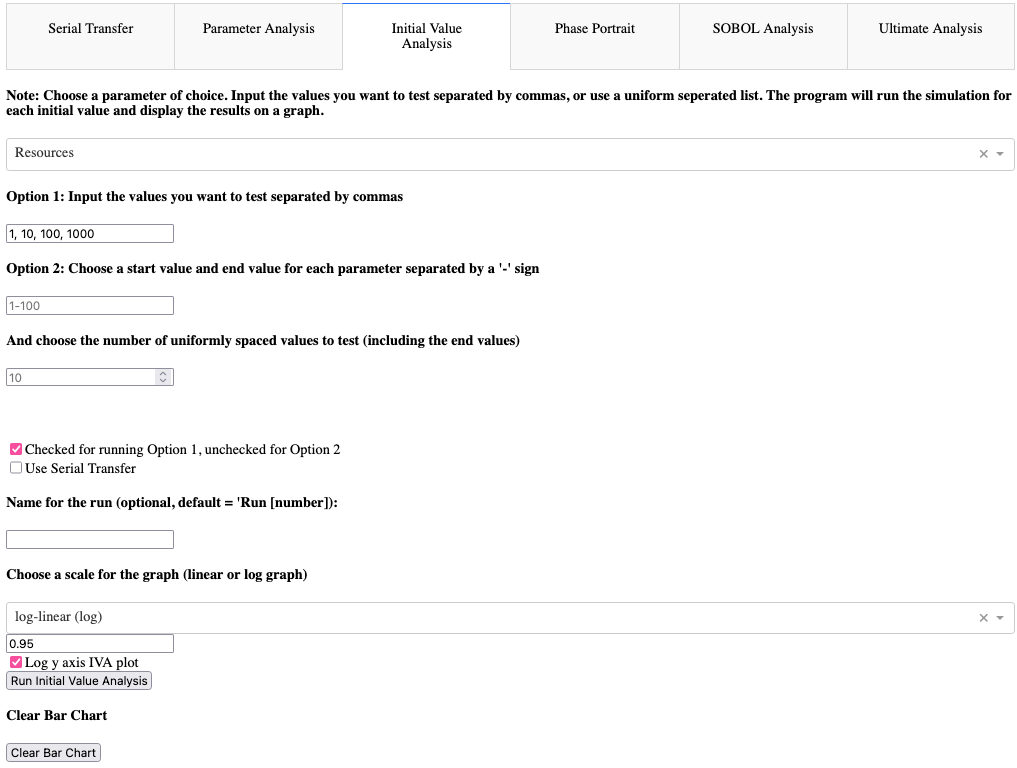
\includegraphics[width=\linewidth]{Screenshots/AdvancedVisualization/initial_value_analysis_settings.png}
        \caption{
            The settings for the initial value analysis tab. 
        }
        \label{fig:ss:av:initial_value_analysis_settings}
        \vspace*{\fill}
    \end{subfigure}
    \hfill
    \begin{subfigure}{0.49\linewidth}
        \centering
        \vspace*{\fill}
        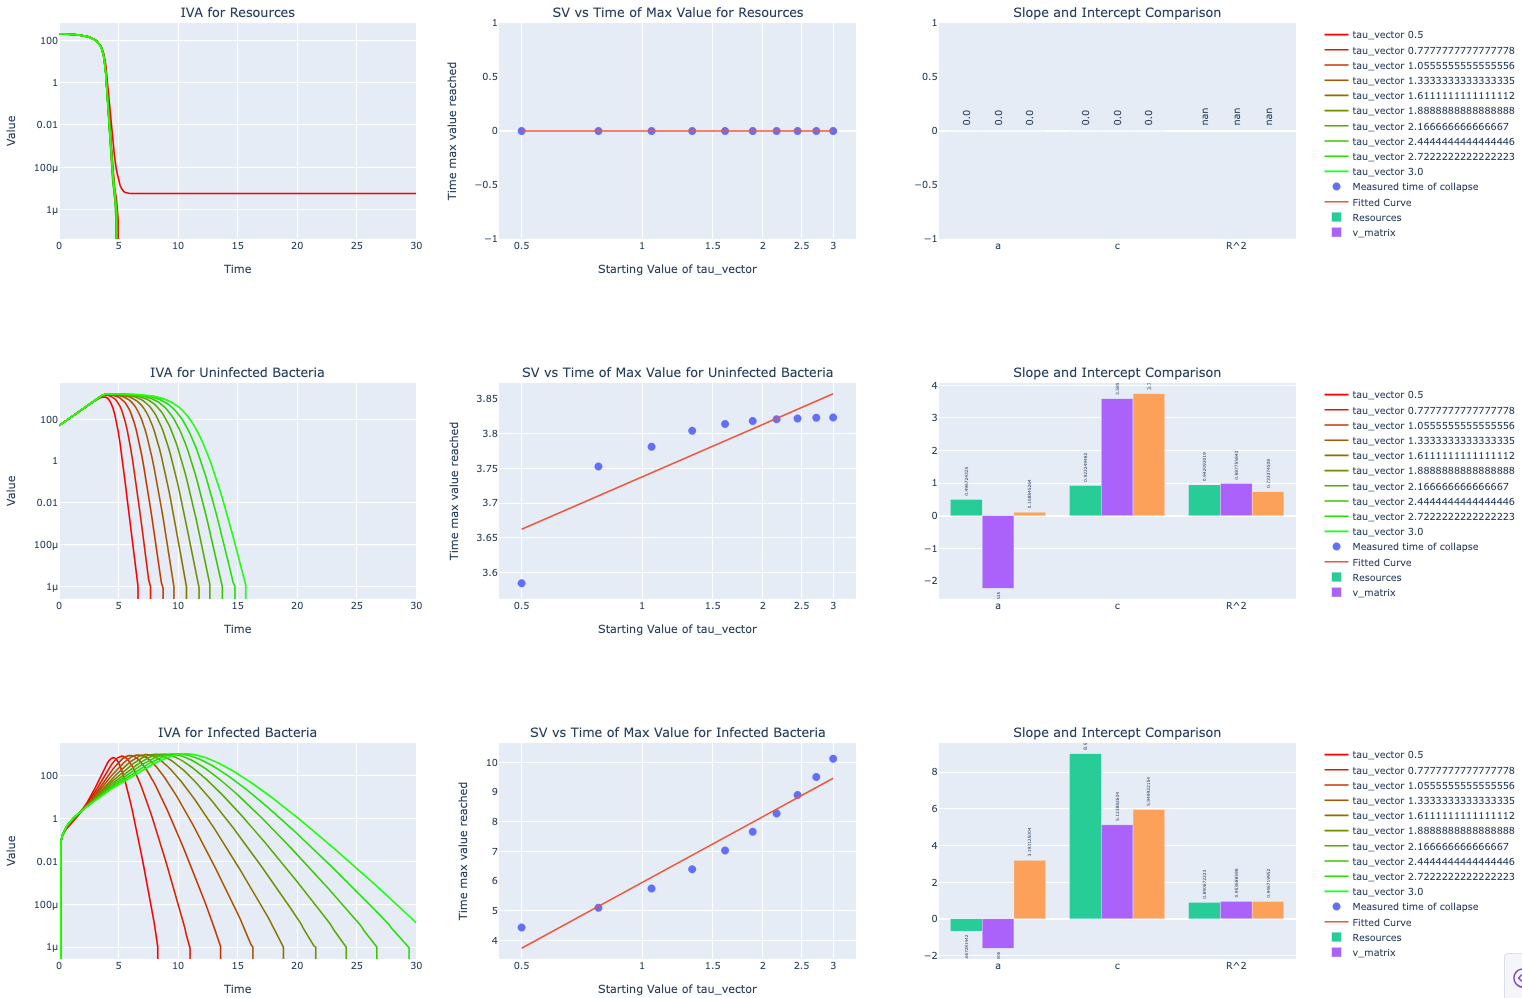
\includegraphics[width=\linewidth]{Screenshots/AdvancedVisualization/initial_value_analysis_run.png}
        \caption{
            An example initial value analysis output. 
        }
        \label{fig:ss:av:initial_value_analysis_run}
        \vspace*{\fill}
    \end{subfigure}
    \caption{Initial value analysis}
\end{figure}

\subsubsection{Phase Portrait}
\label{sec:phase_portrait}
The phase portrait plot allows for the user to analyze how an agent population evolves with respect to the other agent population through time.
Phase portraits indicate how one population increases while the other decreases, and vice versa.
Steady states can be identified and classified as either stable, unstable, or as saddle points.
By comparing different starting points, it is possible to see if the system is chaotic or not.
The setup for the phase portrait can be seen in \Cref{fig:ss:av:phase_portrait_settings}, and a sample output can be seen in \Cref{fig:ss:av:phase_portrait_run}. 

\begin{figure}[h!]
    \centering
    \begin{subfigure}{0.49\linewidth}
        \centering
        \vspace*{\fill}
        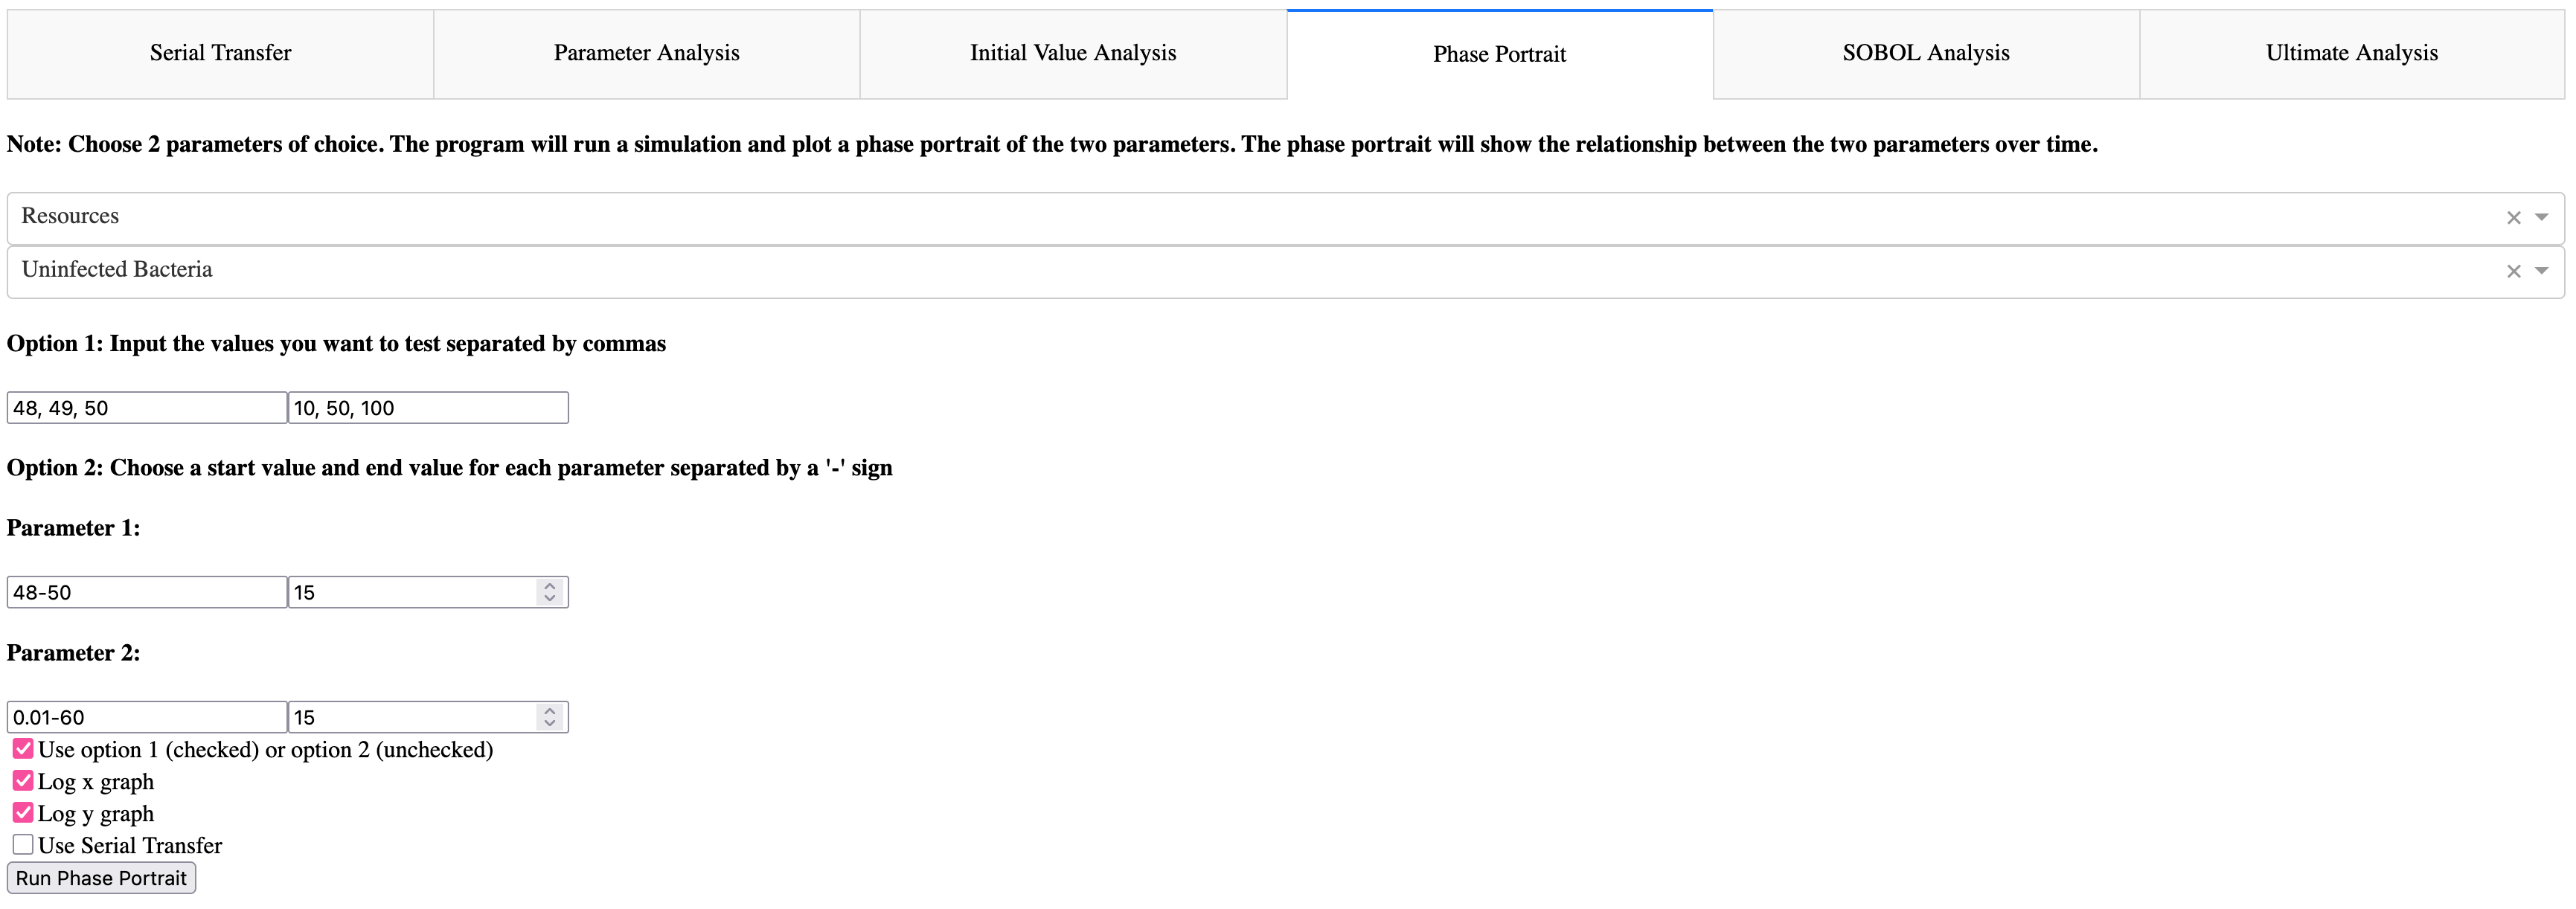
\includegraphics[width=\linewidth]{Screenshots/AdvancedVisualization/phase_portrait_settings.png}
        \caption{
            The user can select two starting values for the initial condition, but they can't choose vector, matrix, or environment settings due to the plot showing the development of agent populations against other agent populations.
            As typical, the user can select their own values or auto-generate values between two values, as well as use a serial transfer option.
            There is also an option to take the logarithm of the x and/or y-axis. 
        }
        \label{fig:ss:av:phase_portrait_settings}
        \vspace*{\fill}
    \end{subfigure}
    \hfill
    \begin{subfigure}{0.49\linewidth}
        \centering
        \vspace*{\fill}
        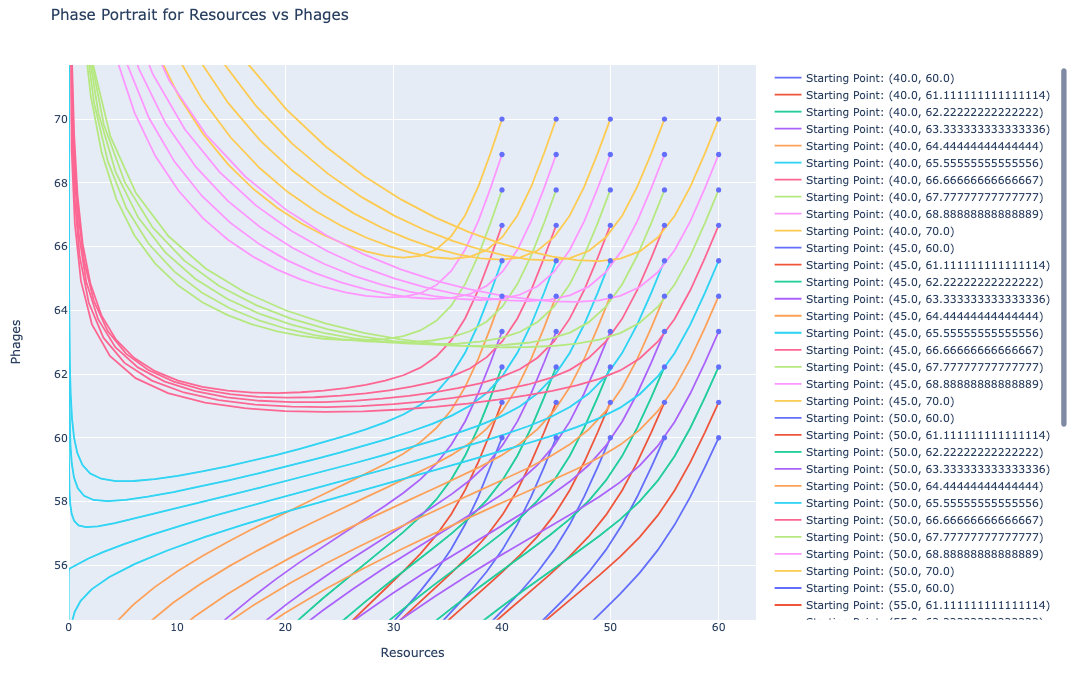
\includegraphics[width=\linewidth]{Screenshots/AdvancedVisualization/phase_portrait_run.png}
        \caption{
            An example run of a phase portrait.
        }
        \label{fig:ss:av:phase_portrait_run}
        \vspace*{\fill}
    \end{subfigure}
    \caption{Phase Portrait}
\end{figure}

\subsubsection{SOBOL Analysis}
\label{sec:SOBOL_analysis}
SOBOL analysis, a variance-based sensitivity analysis, is a method that allows a user to quantify how important an input parameter has on a measured aspect of the output by changing the parameter values of the model and measuring the change in model output.
SOBOL quantifies how much variance in the output can be attributed to a specific parameter and can measure the effect of global, first, and second order sensitivity. 
When a model is viewed as a black-box model, the model can be seen as a function $Y=f(X)$, where $X$ is an input vector of $d$ elements, and $Y$ is a univariate model output.
$X$ is assumed to be independently and uniformly distributed within a hypercube $X_i \in [0, 1]$ for $i=1, \dots d$.
The first order sensitivity measures the output variance of the main affect of parameter $X_i$.
Measuring the effect of varying $X_i$ averaged over other input parameters, and standardized to provide a fractional contribution to the overall output variance.
The first order sensitivity is described as
\[
    S_i = \frac{V_i}{\textit{Var}(Y)}
\] where $V_i = \textit{Var}_{X_i}(\mathbb{E}_{X_{\sim i}}[Y|X_i])$ and where $X_{\sim i}$ represents all the parameters that are not $X_i$.
\newline


The second order index measures the impact of input $X_i$ interacting with $X_j$. For many inputs, this becomes unwieldy to analyze.
The global sensitivity is used to analyze the global sensitivity without evaluating $2^d-1$ indices, and measures the contribution to the output variance of $X_i$, including all variance due to $X_i$s interaction with other variables.
\[
    S_{T_i} = \frac{\mathbb{E}_{X_{\sim i}}[\textit{Var}_{X_i}(Y|X_{\sim i}))}{\textit{Var}(Y)} = 1 - \frac{\textit{Var}_{X_i}(\mathbb{E}_{X_i}[Y|X_{\sim i}])}{\textit{Var}(Y)}
\]
SOBOL can analyze various univariate outputs.
This could be either the average value of an agent population, the variance in population count, the time at the peak of an agent count, the final population value, etc. \newline
SOBOL accepts a list of parameter names and a list of range of values to sample from, which the user can input in the SOBOL settings tab, \Cref{fig:ss:av:SOBOL_analysis_settings}. 
If no values are added, the parameter is not included in the simulation and the default value is instead used. 
The user then needs to select the number of samples to run, using the formula $2^x$, where $x$ is the number they input, and $2^x$ is the number of samples that SOBOL will create and run.
The larger $x$ is, the more accurate the SOBOL analysis results will be, but the more simulations would need to be run. \newline
If the user wants to analyze the second order interactions, then the model will run the system $N(2D+2)$ times with the randomly sampled input values, where $N$ is a multiple of 2, and $D$ is the number of parameters being tested.
Otherwise, if 2nd order is not chosen, the model is run $N(D+2)$ times.
Due to the randomness of the sampling method, the user can, but does not need to, submit a seed value. 


Three SOBOL analyses are included by default in the dashboard, as shown in \Cref{fig:ss:av:SOBOL_analysis_run}.
An analysis of the final value of the simulation, the average population count, and the variance in population count.
The global and first sensitivity are shown next to one another, and each sub-row within a plot represents each agent type. 
The proportion of the global and local sensitivity can be seen for each agent type and each parameter.

\begin{figure}[h!]
    \centering
    \begin{subfigure}{0.49\linewidth}
        \centering
        \vspace*{\fill}
        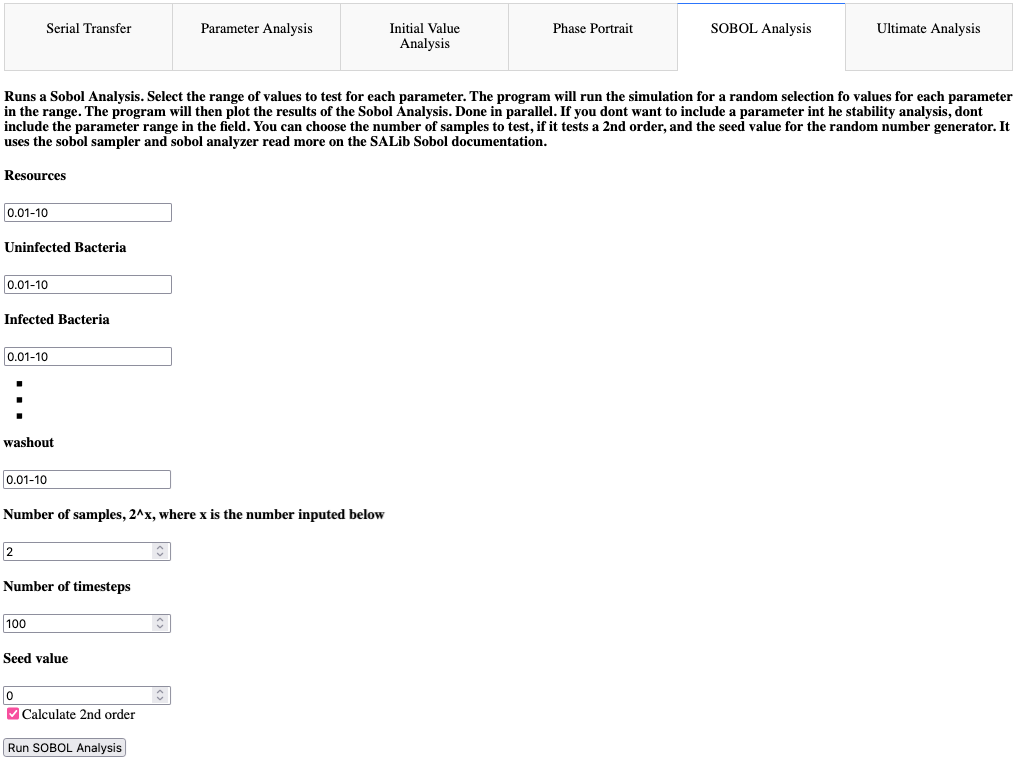
\includegraphics[width=\linewidth]{Screenshots/AdvancedVisualization/SOBOL_analysis_settings.png}
        \caption{
            The SOBOL settings tab. 
        }
        \label{fig:ss:av:SOBOL_analysis_settings}
        \vspace*{\fill}
    \end{subfigure}
    \hfill
    \begin{subfigure}{0.49\linewidth}
        \centering
        \vspace*{\fill}
        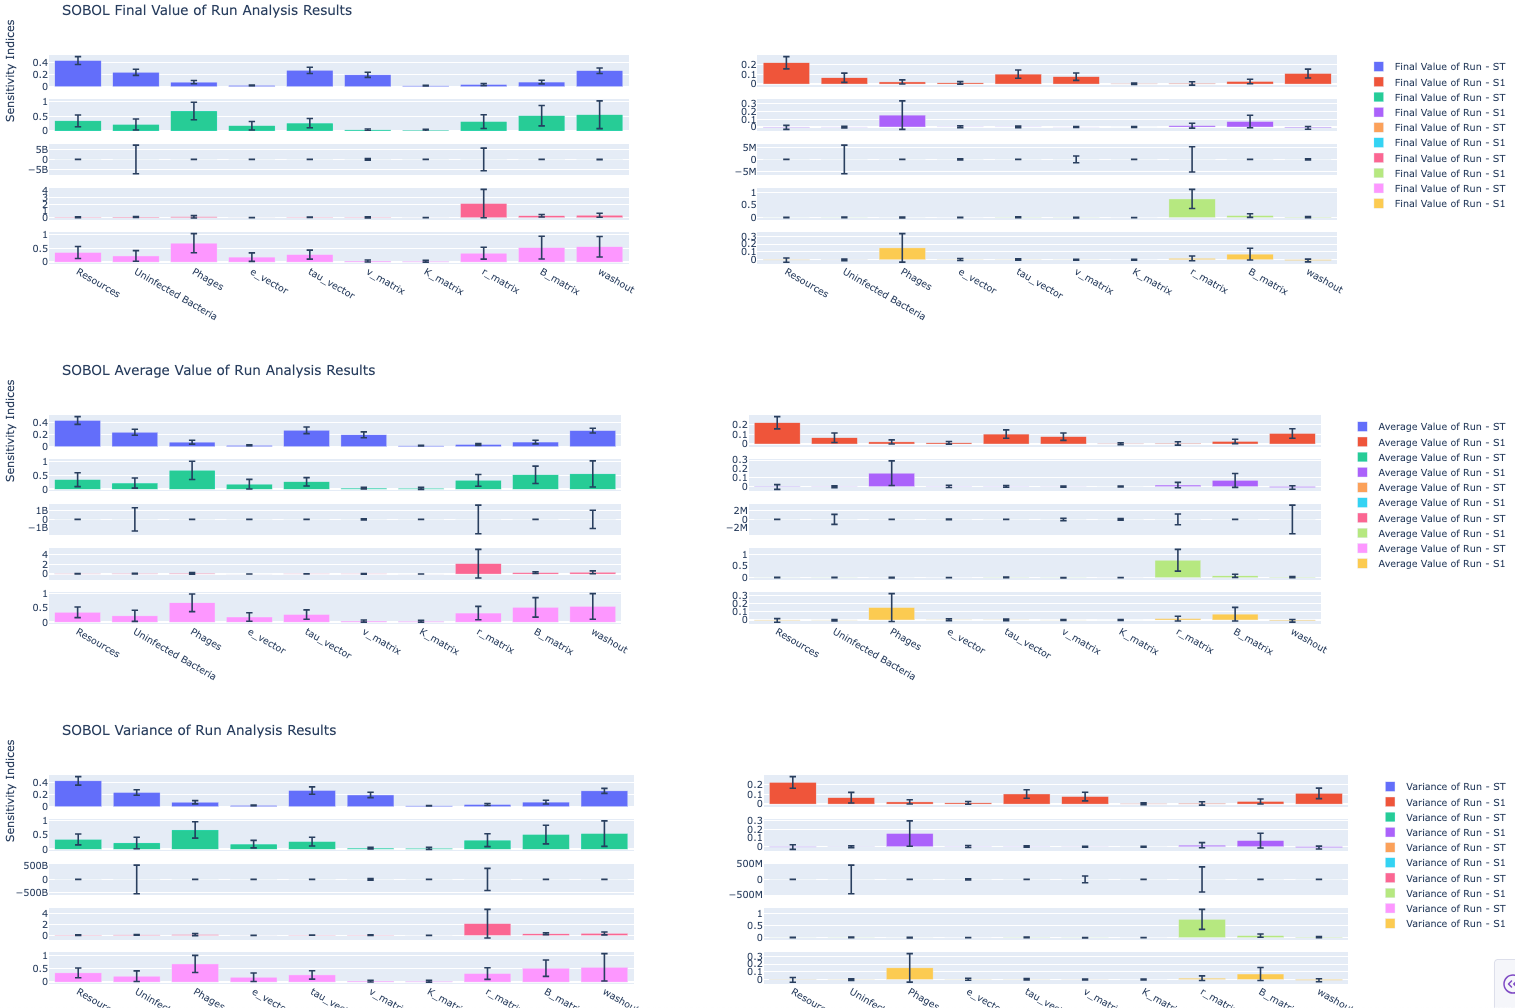
\includegraphics[width=\linewidth]{Screenshots/AdvancedVisualization/SOBOL_analysis_run.png}
        \caption{
            The output that can be expected from SOBOL. 
        }
        \label{fig:ss:av:SOBOL_analysis_run}
        \vspace*{\fill}
    \end{subfigure}
    \caption{SOBOL variance analysis}
\end{figure}

\subsubsection{Ultimate Analysis}
\label{sec:ultimate_analysis}
The Ultimate Analysis section does not produce any visualizations or analysis, but instead allows for the user to define which initial conditions and parameter values they want to run a simulation on.
The solver will iterate over every single parameter input possibility and save the results in a \textit{.parquet} file.
Similarly to the other sections, the user can specify a start and end value, along with the number of values to generate evenly spaced within that range, including both the start and end values.
\newline
Using Dask and the saved \textit{.parquet} file, the user can query for specific runs, for example runs where a parameter value was greater than 0.05, and use the simulation data to create their own plots.
\begin{figure}
    \centering
    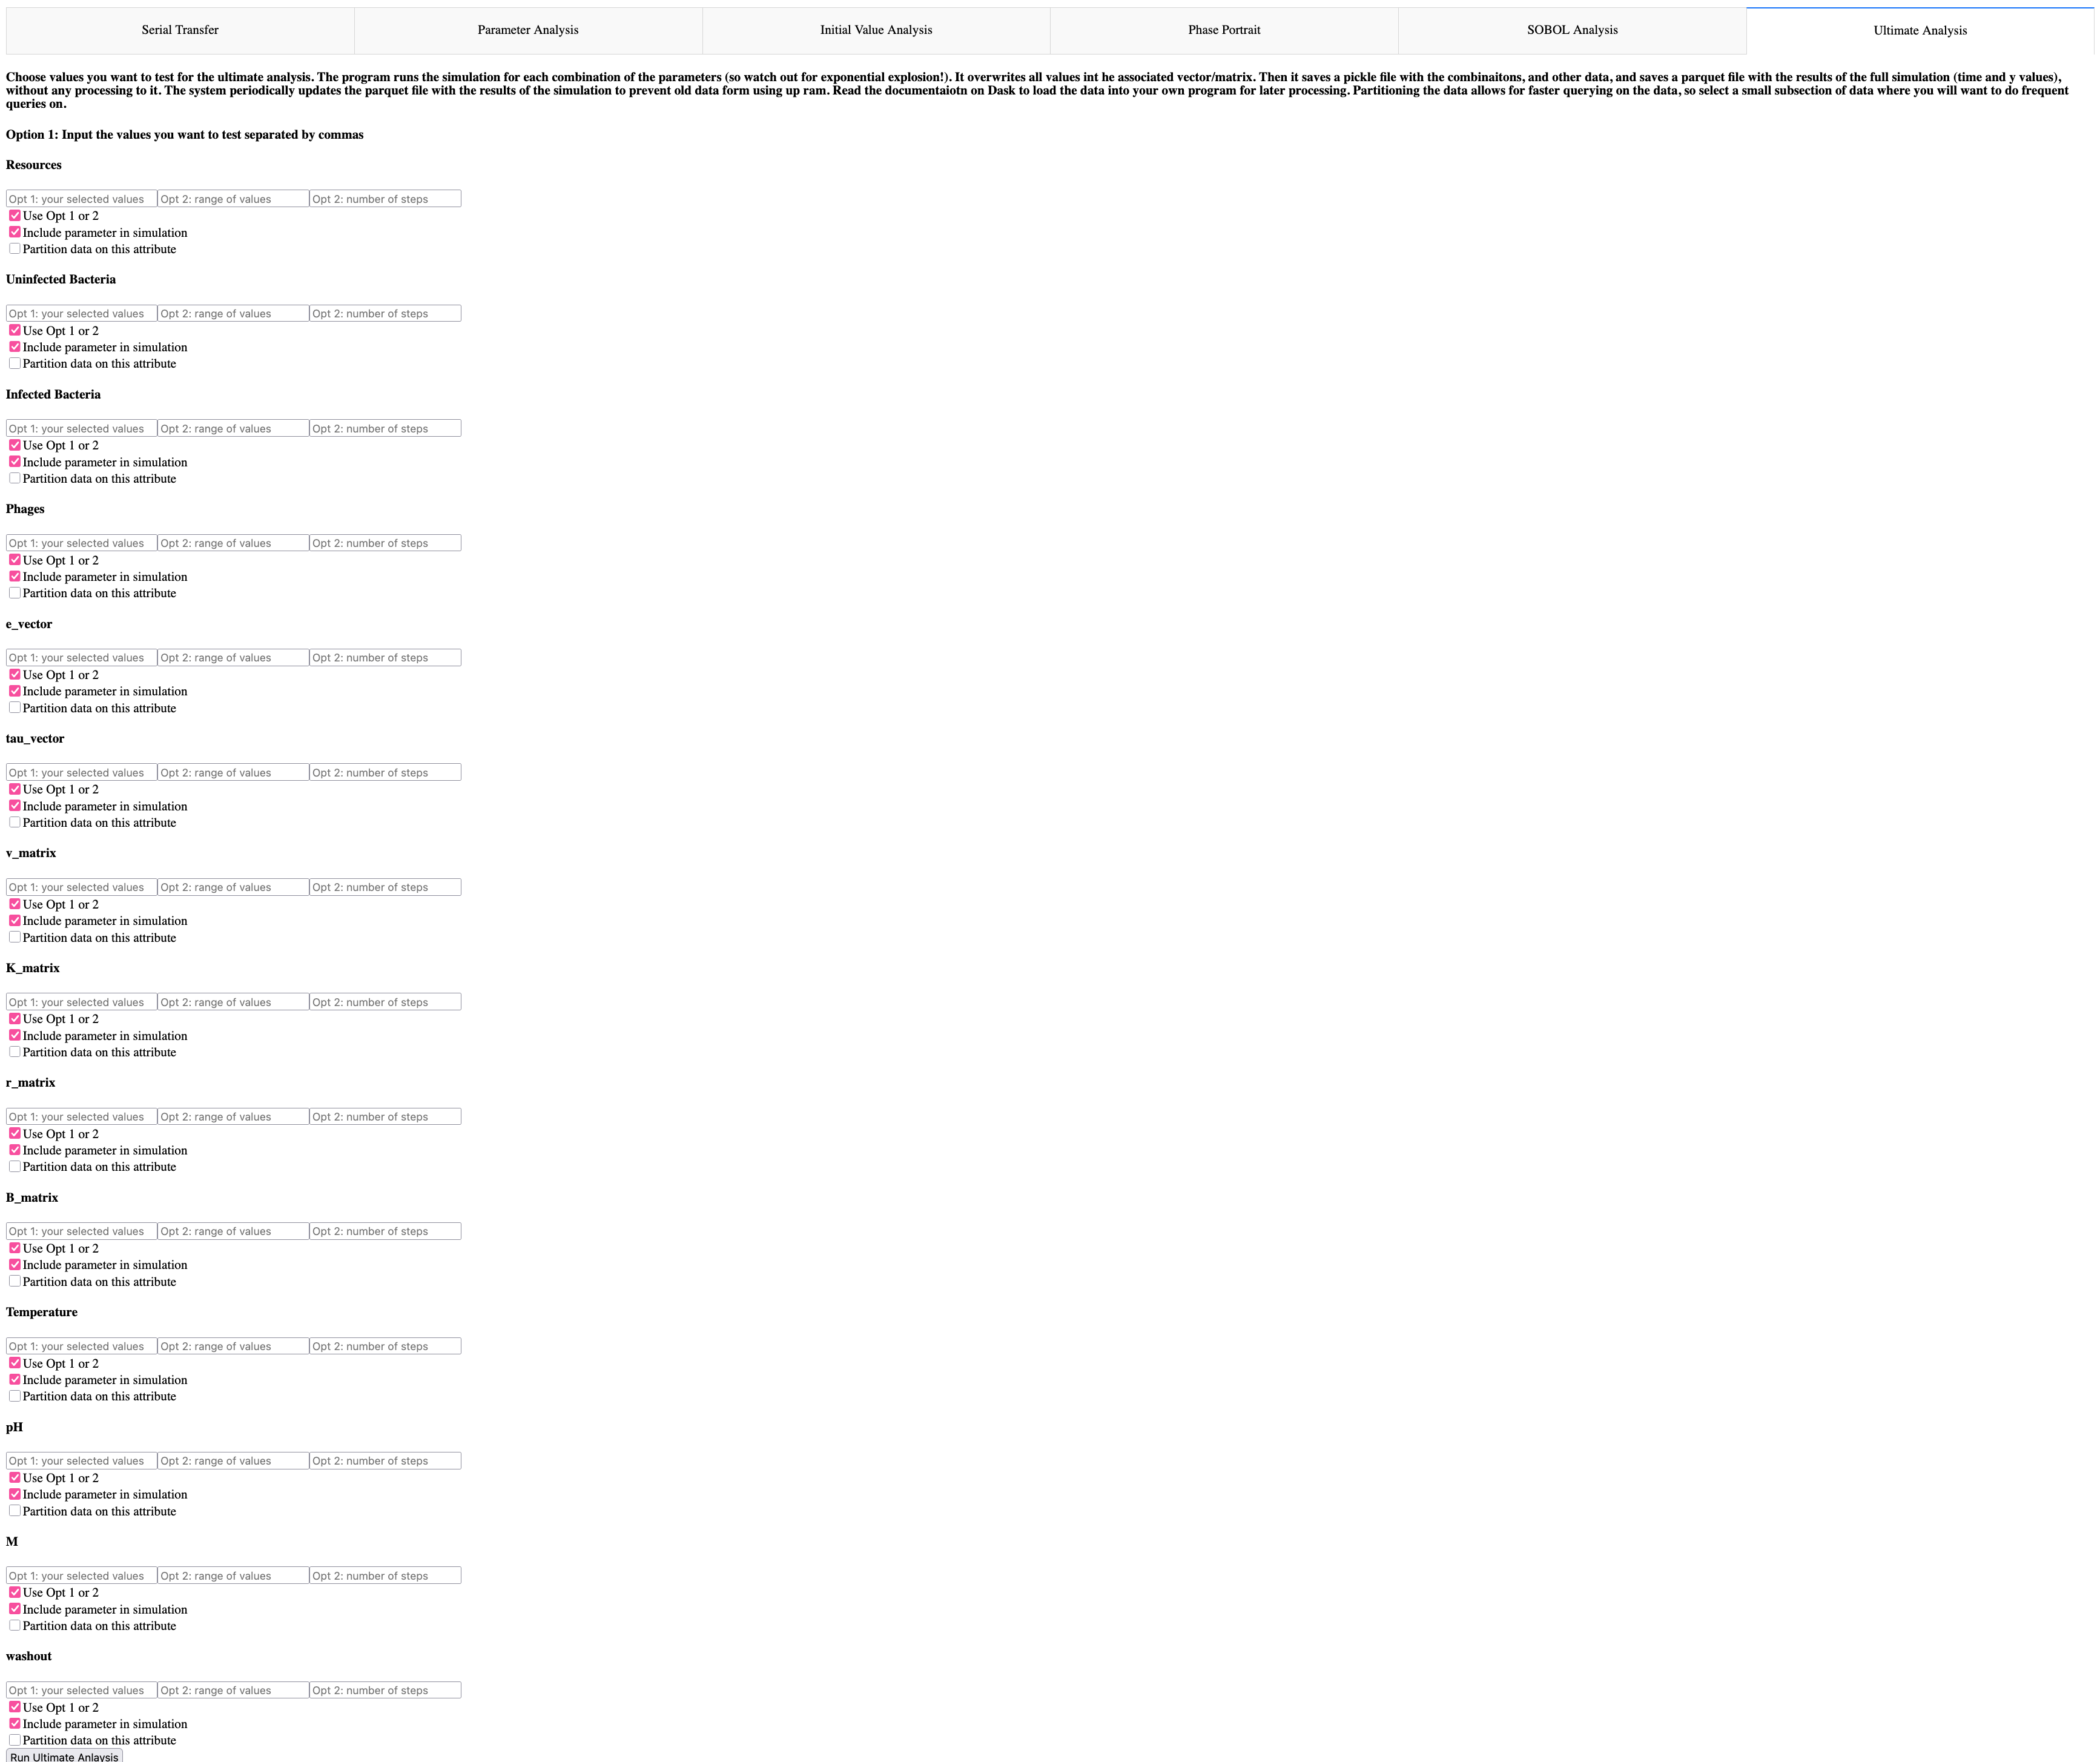
\includegraphics[width=1\linewidth]{Screenshots/AdvancedVisualization/ultimate_analysis_settings.png}
    \caption{
        The ultimate analysis setup tab. 
    }
    \label{fig:ss:av:ultimate_analysis_settings}
\end{figure}


\subsubsection{Custom Advanced Analyses and Visualizations}
\label{sec:custom_analysis}
As the dashboard can not create a graph for every situation, or analyze every situation, Ultimate Analysis (\Cref{sec:ultimate_analysis}) can be used to run and download the simulation data to the disk to create later create your own custom visualizations. 
Depending on the used model, different behavior might appear, for example the population count can exhibit cyclic behavior. 
A custom visualization would then perform a Fourier transformation to obtain the predominant frequencies. 

\subsection{Interaction Network}
A flowchart of the interactions between the user and systems can be seen in \Cref{AppendixC}. 

\section{The Golden Model}
\label{sec:golden_model}
In this report, the default model, called the “Golden model“ \cite{gengUsingBacterialPopulation2024} that will be used for all simulations is as follows:

\begin{align}
    \frac{dR}{dt} &= -e \cdot g(R)\cdot (U + \sum_{i=1}^{M} I_M)\\
    \frac{dU}{dt} &= g(N)\cdot U - r\cdot U \cdot P\\
    \frac{dI_1}{dt} &= r\cdot U \cdot P - \frac{M}{\tau}\cdot I_1 \\
    \frac{dI_k}{dt} &= \frac{M}{\tau}(I_{k-1}-I_k) \text{ for } k=2, \dots, M \\
    \frac{dP}{dt} &= \beta \cdot\frac{M}{\tau} \cdot I_M - r\cdot(U + \sum_{i=1}^{M} I_M)\cdot P \\
    g(N) &= \frac{v\cdot N}{N + K}
\end{align}where $N$ is resources, $U$ is uninfected bacteria, $I_{1, \dots, M}$ is the infected stage of the bacteria, and $P$ is the phage population. \newline
The model describes three biological processes, cell consumption of resources and growing, phage/cell encounters and infection, and cell lysis. 
The cell growth process is described by $g(N)$, the instantaneous growth rate dependent on the Monod equation, where $v$ is the maximal growth rate and $K$ is the Monod constant. 
The consumption rate of a resource by a bacteria is $e$. \newline
Once infected by a phage, cells go through $M$ stages of infection $I_1, \dots, I_M$ before lysing, with equal transition probability $\frac{M}{\tau}$ from state $I_k$ to state $I_{k+1}$. The probability of a successful infection of a cell is $r$. \newline
After a bacteria lyses after stage $I_M$, $B$ phages are releases, the burst size of the phage. \newline 

However this model is specifically designed for a $1\times 1 \times 1$ model. 
In order to adapt this model to fit an $p \times b \times r$ model, the model needs to be adapted. 
There are other changes that can be made, to the model, for example by adding a washin rate $\omega^{i}$, where resources are constantly being introduced, such as in a chemostat, and a washout rate $\omega^{o}$ where phages, bacteria, and resources are being washed out. 

\subsection{The Adapted Golden Model}
\label{sec:adapted_golden_model}
\begin{align}
    \frac{dN_n}{dt} &= \sum_{b \in B} -e_{b, n} \cdot g(N_n, b)\cdot (U_b + \sum_{i=1}^{M} I_{i_b}) + w^i_n - w^o \cdot N_n\\
    \frac{dU_b}{dt} &= U_b \cdot \sum_{b \in B} g(N_n, b)\cdot - U_b \cdot (\sum_{p \in P} r_{p, b} \cdot P_p) - w^o \cdot U_b\\
    \frac{dI_{1_b}}{dt} &= U_b \cdot (\sum_{p \in P}r_{p, b} \cdot P_p) - \frac{M}{\tau_b}\cdot I_{1_b} - w^o \cdot I_{1_b}\\
    \frac{dI_{k_b}}{dt} &= \frac{M}{\tau}(I_{k-1_b}-I_{k_b}) - w^o \cdot I_{k_b}\text{ for } k=2, \dots, M \\
    \frac{dP_p}{dt} &= \beta_{p, b}\cdot\frac{M}{\tau_b} \cdot I_{M_b} - r_{p, b}\cdot(U_b + \sum_{i=1}^{M} I_{M_b})\cdot P_p - w^o \cdot P_p\\
    g(N_n, b) &= \frac{v_{b, n} \cdot N_n}{N_n + K_{b, n}}
\end{align}. 


\section{Software Used and Packages}
The program was created exclusively in Python, and makes extensive usages of various packages, ranging from the standard scientific packages such as NumPy and SciPy to more niche packages such as pickle and SALib. \newline

The graphical tool uses Tkinter acting as the front end, handling the user inputs, while NetworkX stores the graph and contains the attribute data. 
The GUI tool also uses Matplotlib to create the figure of the graph to display to the user in the GUI tool. \newline

The simulation framework, the backend of the modelling, makes extensive usage of SciPy's \textit{solve\_ivp()} to create the ODE data. 
It also makes light usage of NetworkX to load the graph, as it initially takes a graph as an input, and light usage of NumPy to setup the parameters at startup. \newline 

The visualization part makes heavily usage of Dash and Plotly. 
Dash acts as the server and is used for displaying the HTML aspect of the frontend and dealing with any input and output. 
Upon choosing parameter values and clicking on “submit“, Dash registers the activity and calls the function registered to the button, sending data such as parameter values and options like "log x-axis" form the frontend to the backend server. 
In the backend, the various inputs are handled, like changing the input string "0.05, 0.1, 0.15, 0.2" provided by the user into an iterable list [0.05, 0.1, 0.15, 0.2] that the simulation framework can iterate over to vary the parameter value. 
Then a call to the simulation solver is done. \newline 

If there are many simulations to run through, in the case of SOBOL (\ref{sec:SOBOL_analysis}) or ultimate analysis (\ref{sec:ultimate_analysis}), then an intermediate call to a parallel computing library Joblib is called, where Joblib parallelizes the for-loop to compute the simulations in parallel. 
The ultimate analysis makes use of pandas to store the data as a dataframe to then be stored as a \textit{.parquet} file. 
To effectively load the data saved from the ultimate analysis section, the user can use Dask to query and load large datasets into memory. \newline 
SOBOL makes use of the SALib library to sample and analyze the parameter input. 
Both the ultimate analysis and SOBOL also save a \textit{.pickle} file containing a dictionary with the parameter values tested,and other important information regarding the simulation in question. \newline
The initial value analysis visualization (\Cref{sec:initial_value_analysis}) uses SciPy's \textit{curve\_fit()} function to curve fit the points in the middle plot (\Cref{fig:ss:av:initial_value_analysis_run}). 

Other packages that are used include Pandas, collections, copy, warnings, itertools, os, datetime, json, gc, and time. 